\chapter{Ergebnisse}
\label{chap:ergebnisse} Dieses Kapitel präsentiert alle Ergebnisse, die in
dieser Arbeit erzielt wurde. Dabei spielen nicht nur die erfolgreichen Ziele eine
Rolle, sondern auch die Misserfolge. Zunächst wird die entwickelte Erweiterung in
seiner finalen Form beschrieben, gefolgt von einer Darstellung der zentralen
Funktionen. Anschließend wird auf die Konzeptionen und Umsetzungen der verschiedenen
Teile eingegangen. Abschließend soll die Performance und die verschiedenen
Anwendungsszenarien genauer analysiert werden. Daraus ergeben sich auch Limitierungen
für die Software. Mit diesen erstellten Analysen kann unter Berücksichtigung
eine Aussage bezogen auf die Forschungsfrage gestellt werden.
% ---------------------------------------------------------------------------------------

\section{Tooth Analyser}
\label{sec:tooth_analyser} Im Rahmen dieser vorliegenden Arbeit ist eine 3D
Slicer Extension entstanden, die den Namen Tooth Analyser trägt und für die Forschung
im Dentalbereich eingesetzt wird. In erster Linie können mit diesem Plugin Micro
CT Aufnahmen anatomisch segmentiert werden. Das Modul schmiegt sich wie alle anderen
Module gut in die Kernanwendung ein und ist auch für die aktuelle stabile Version
von Slicer (v5.8.0) verfügbar. Neben der eigentlichen Implementierung ist auch
ein Logo für das Plugin entstanden, das es nach außen repräsentiert. Die
Abbildung \ref{fig:logo_tooth_analyser} zeigt dies.

\begin{figure}[h]
	\centering
	
\includegraphics[width=0.9\textwidth]{img/SlicerToothAnalyser.png}
	\caption{Logo der 3D Slicer Erweiterung "Tooth Analyser", welche im Rahmen dieser
	Arbeit entwickelt wurde. Logodesign: Dr. Elias Walter}
	\label{fig:logo_tooth_analyser}
\end{figure}

Des Emblem des Tooth Analyser bildet einen Zahn ab, dessen Hauptsegmenten (Schmelz,
Dentin, Pulpa) mit den unterschiedlichen Farben (grün, gelb, orange)
visualisiert werden. Dies verdeutlicht die Analogie zur anatomischen Segmentierung
und lässt gleich vermuten, dass sich dieses Modul mit einer Segmentierung
beschäftigt. Der Untertitel deutet konkret auf Micro \ac{CT} Aufnahmen hin. Wurde
der Tooth Analyser installiert, so ist er über den Menüpunkt Module in Slicer
auswählbar. Hier wird er in dem Unterpunkt \textit{Segmentierung} eingruppiert, was
ein weiteres Indiz auf die grobe Funktionalität liefert. Wird also der Tooth
Analyser gestartet so erhält man die Ansicht der Kernanwendung mit der
Entsprechenden \ac{UI}. Die Abbildung \ref{fig:tooth_analyser_start_up} soll
genau diese Ansicht verdeutlichen

\begin{figure}[h]
	\centering
	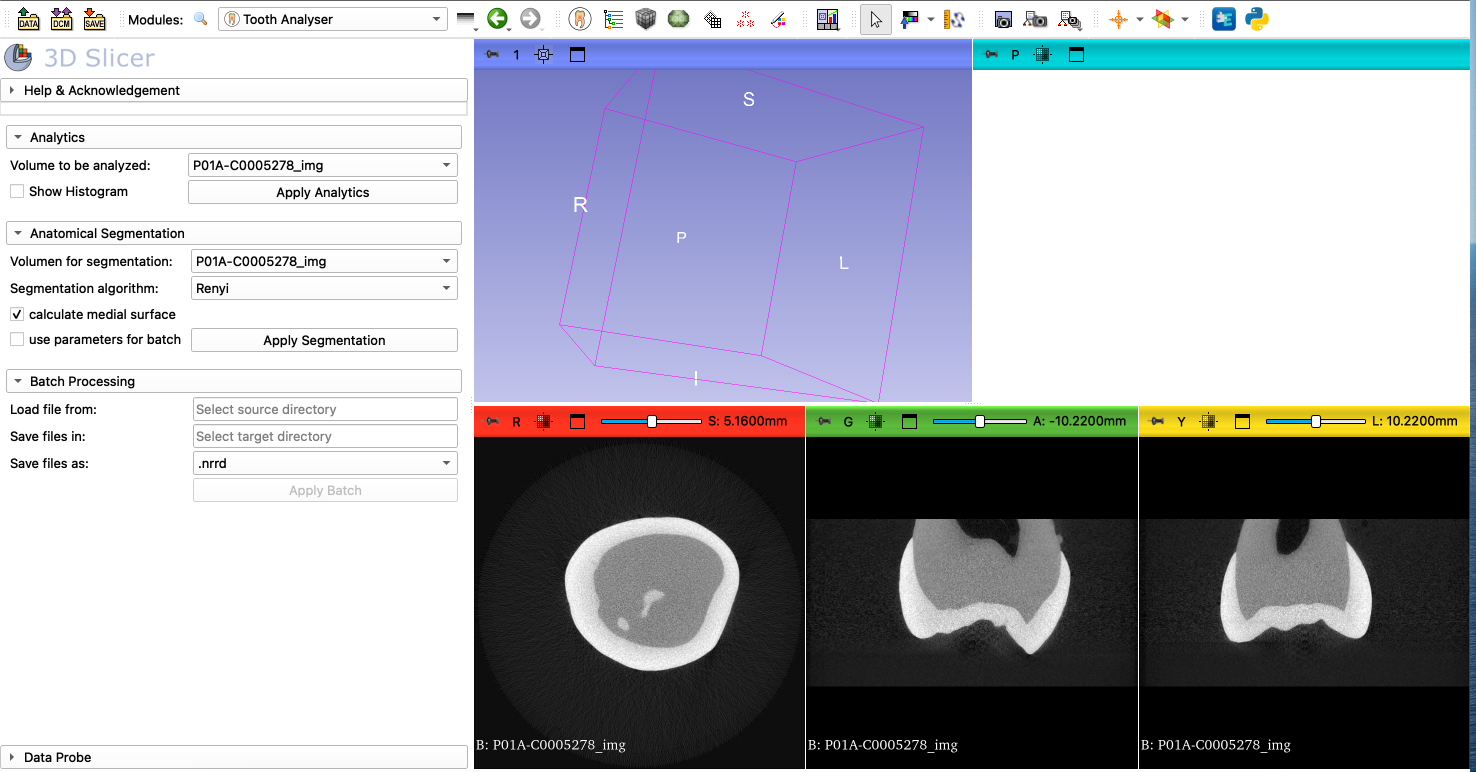
\includegraphics[scale=0.2, width=\textwidth]{img/toothAnalyserStarUp.png}
	\caption{Startansicht der Erweiterung Tooth Analyser nach dem ersten Aufruf}
	\label{fig:tooth_analyser_start_up}
\end{figure}

Die Ansicht zeigt die Kernanwendung (rechts die verschiedenen Fenster) und die
\ac{UI} des jeweiligen Moduls. Die Kernanwendung kann auch als Szene beschrieben
werden und übernimmt alle generischen Handhabungen der Bilder. Neben den Szenen ist
auch immer eine Sidebar zu sehen, welche die \ac{UI} des jeweiligen Moduls abbildet.
Im Falle der Abbildung \ref{fig:tooth_analyser_start_up} ist es die \ac{UI} des Tooth
Analyser. Das manuelle Laden eines Bildes in die Szene ist Teil der Slicer
Kernanwendung und nicht teil der Modullogik. Das bereits geladene Bild ist demnach
unabhängig von der Slicer Erweiterung entstanden. Betrachtet man die
Benutzerschnittstelle genauer, so fällt sofort auf, dass diese in vier Bereiche
unterteilt ist. Diese Aufteilung in Bereiche ist ein Ergebnis der Literaturrecherche
und eine gute Konvention in der Welt von 3D Slicer. Der Bereich \textit{Help and
Acknowledgement} stellt Hilfen und Informationen über das Modul bereit. Über
diesen Abschnitt ist auch die offizielle Dokumentation über dieses Modul
erreichbar. Zu Beachten ist, dass dieser Bereich nicht eigens für den Tooth
Analyser entwickelt wurde. Es handelt sich hier um eine Funktionalität, die
automatisch allen \ac{SEM} zur Verfügung steht. Bei den übrigen Abschnitten
handelt es sich im Features die spezifische für den Tooth Analyser entwickelt
wurden. Bevor genauer auf die Funktionalitäten des Tooth Analyser eingegangen wird,
sei zunächst auf die Abbildung \ref{fig:tooth_analyser_full_view} verwiesen, welche
die Ergebnisansicht zeigt.

\begin{figure}[h]
	\centering
	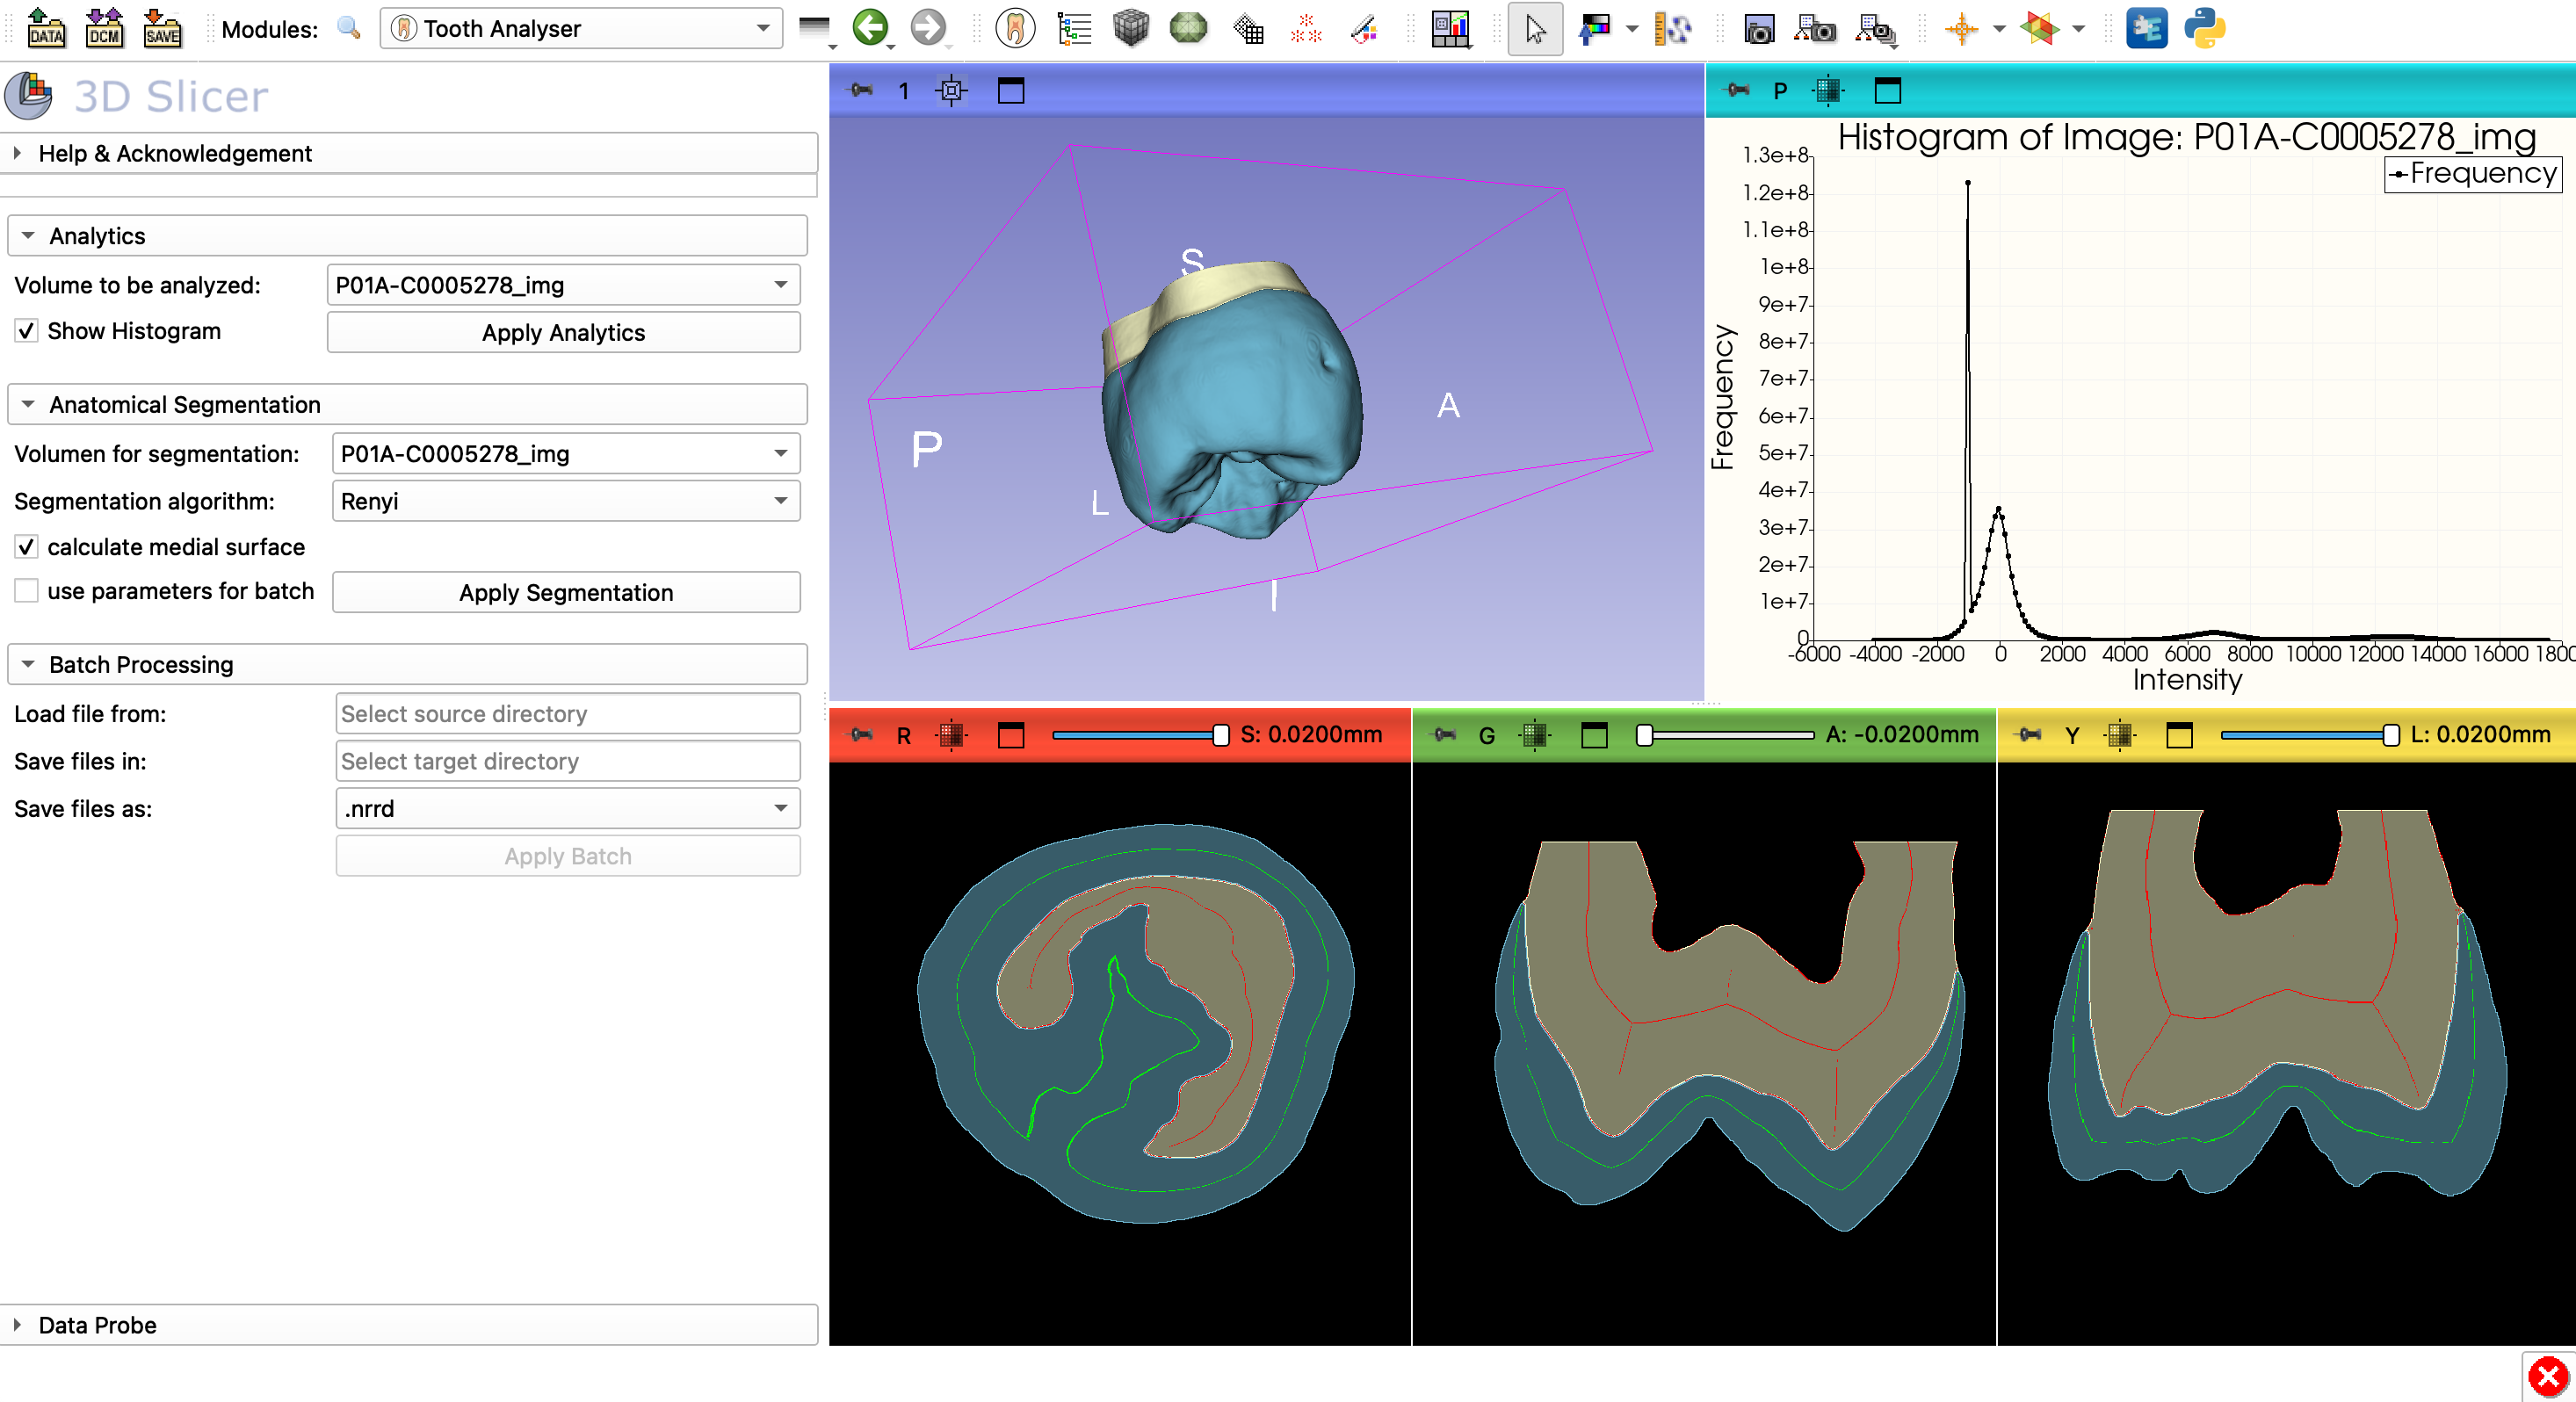
\includegraphics[scale=0.2, width=\textwidth]{img/toothAnalyserFullView.png}
	\caption{Ergebnisansicht der Erweiterung Tooth Analyser, nachdem die Analysen und
	die anatomische Segmentierung erstellt wurden.}
	\label{fig:tooth_analyser_full_view}
\end{figure}

Der Analysebereich des Tooth Analyser ermöglicht es das Histogramm eines
gegebenen Bildes zu erstellen. Dies ist besonders interessant, wenn ein
Algorithmus für die anatomische Segmentierung ausgewählt werden muss. Diese Algorithmen
sind Schwellwertverfahren, die auf das Histogramm eines Bildes basieren, um es zu
segmentieren. Das erstellte Histogramm ist rechts oben in der Abbildung
\ref{fig:tooth_analyser_full_view} zu erkennen. Es wird in einem Plot-Node dargestellt
und kann über diesen auch verändert werden. Hierzu ist die Pinnnadel im Fenster
des Plot-Node zu wählen. Durch die Speicherfunktion der Kernanwendung kann der Plot
auch problemlos gespeichert werden. Bevor die Analysen erstellt werden können, müssen
Parametereinstellungen gewählt werden. Hierbei ist der wichtigste Parameter der,
indem das konkrete Bild ausgewählt wird. Bei diesem Parameter handelt es sich um
ein Dropdown, indem nur Bilder mit dem Typ \texttt{vtkMRMLScalarVolumeNode}
ausgewählt werden können. Dies trägt zur Stabilität und Ausfallsicherheit des Systems
bei und sorgt dafür, dass nicht jedes beliebige Bild geladen werden kann. Ist keine
\ac{CT} Aufnahme ausgewählt, so bleibt der Button zum Starten der Analysen deaktiviert.
Wird ein Bild in die Szene geladen, während der Parameter für das zu analysierende
Bild leer ist, wählt der Tooth Analyser automatisch das Bild aus, dass als Erstes
in die Szene geladen wurde. So spart der Benutzer einige Klicks. Durch die Checkbox
\textit{Show Histogram} wird der Erweiterung signalisiert das beim Starten der
Analysen ein Histogramm des übergebenen Bildes erstellt werden soll.

Die Hauptfunktionalität des Tooth Analyser ist die anatomische Segmentierung
welche in Kapitel \ref{sec:verwwandte_arbeit} detailliert erläutert wurde. Die konkreten
Ergebnisse dieser Segmentierung sind in der Abbildung \ref{fig:tooth_analyser_full_view}
in den Fenstern (blau, rot, grün, gelb) zu sehen. Neben der eigentlichen Segmentierung
sind auch hier die medialen Flächen für die Segmente Dentin (rot) und Schmelz (grün)
gut sichtbar. Hinzu kommt ein \ac{3D} Modell, das auf Basis der erstellten
Segmentierung generiert wurde und nur der Visualisierung dient. Ein Abspeichern dieses
3D Modells als Netz ist nicht möglich. Um überhaupt eine anatomische
Segmentierung eines Zahnes erstellen zu können, sieht der Algorithmus zunächst drei
Parameter vor, die eingestellt werden müssen. Um die Komplexität gering zu halten,
wurde bewusst auf viele Parameter verzichtet. Ähnlich wie bei den Analysen ist auch
hier die Wahl des zu segmentierenden Volumens der entscheidende Parameter.
Dessen Bedeutung gleicht der Analysen, insbesondere in Bezug auf das Verhalten.
Damit schnell ein Ergebnis generiert werden kann, wurde für die übrigen zwei Parameter
eine Vorauswahl definiert, die zum vollen Ergebnisumfang des Tools führt. So ergibt
sich die Situation, das nach dem Laden eines \ac{CT}s in die Szene nur auf den
Button für das Ausführen gedrückt werden muss, damit eine anatomische Segmentierung
erstellt wird. Dies nimmt dem Benutzer viel Arbeit ab und sorgt für eine gut \ac{UX}.
Sind jedoch Einstellungen in den Parametern gewünscht, so können diese natürlich
getätigt werden. Über den Parameter \textit{Segmentation algorithm} kann das entsprechenden
Schwellwertverfahren gewählt werden, mit dem der Zahn segmentiert werden soll. Dies
mag nur geringfügig eine Änderung auf die Ergebnismenge ausmachen, kann aber
dennoch wichtig sein. Die Checkbox \textit{calculate medial surface} ermöglicht
eine optionale Erstellung der medialen Flächen. Wird diese Funktion ohnehin nicht
gebraucht, so kann diese hier ausgelassen werden und damit Laufzeit eingespart
werden.

Die letzte Funktionalität, die geboten wird, stellt kein neues Verfahren dar, sondern
nur eine andere Art der Ausführung. Die Rede ist hier von einem Batch Modus, der
nicht nur ein Bild segmentiert, sondern das Verfahren der anatomischen
Segmentierung auf eine ganze Reihe an Bildern anwendet. Um diesen Modus aktiv zu
schalten, muss neben den Parametern im Abschnitt \textit{batch} auch die Checkbox
\textit{use parameters for batch} aktiviert werden. Der Tooth Analyser überträgt
dann die aktuellen Parametereinstellungen der anatomischen Segmentierung an den Batch
Modus. Um dann den Batch Modus ausführen zu können, müssen noch zwei Pfade angegeben
werden, die jeweils zu einem Ordner führen. Diese beiden Pfade teilen sich auf in
\textit{source} und \textit{target} und geben an, wo die Daten liegen, die segmentiert
werden soll und wo die segmentierten Daten auf der Festplatte gespeichert werden.
Abschließend ist hier noch zu wählen in welchem Format die erstellten Daten
abgespeichert werden sollen. Bei diesem Feature ist zu beachten, dass nach
Erfolgreichem ausführen keine Daten in der Slicer Szene geladen werden. Der Prozess
läuft im Hintergrund und ist bis auf die Parametereinstellung über die UI komplett
getrennt von Slicer. Nach Ende des Batch Modus wird in dem angegebenen
Zielordner ein Unterordner erstellt, der alle Dateien der segmentierten Bilder enthält.
Hierfür sieht der Tooth Analyser weitere Unterordner für jedes segmentierte Bild
vor. Ein automatisches Laden aller segmentierten Bilder nach dem Batch Prozess ist
nicht implementiert, sodass der erstellte Ordner mit allen Segmentierungsdaten
manuell über den Import geladen werden muss.

Wird nun eines der bereitgestellten Verfahren ausgeführt, so wechselt der Tooth Analyser
in einen sogenannten \textit{Processing Mode}. Dieser soll in erster Linie dem Benutzer
signalisieren, dass aktuell ein Prozess ausgeführt wird. Hierzu sei auf die Abbildung
\ref{fig:processing_mode} verwiesen.

\begin{figure}[h]
	\centering
	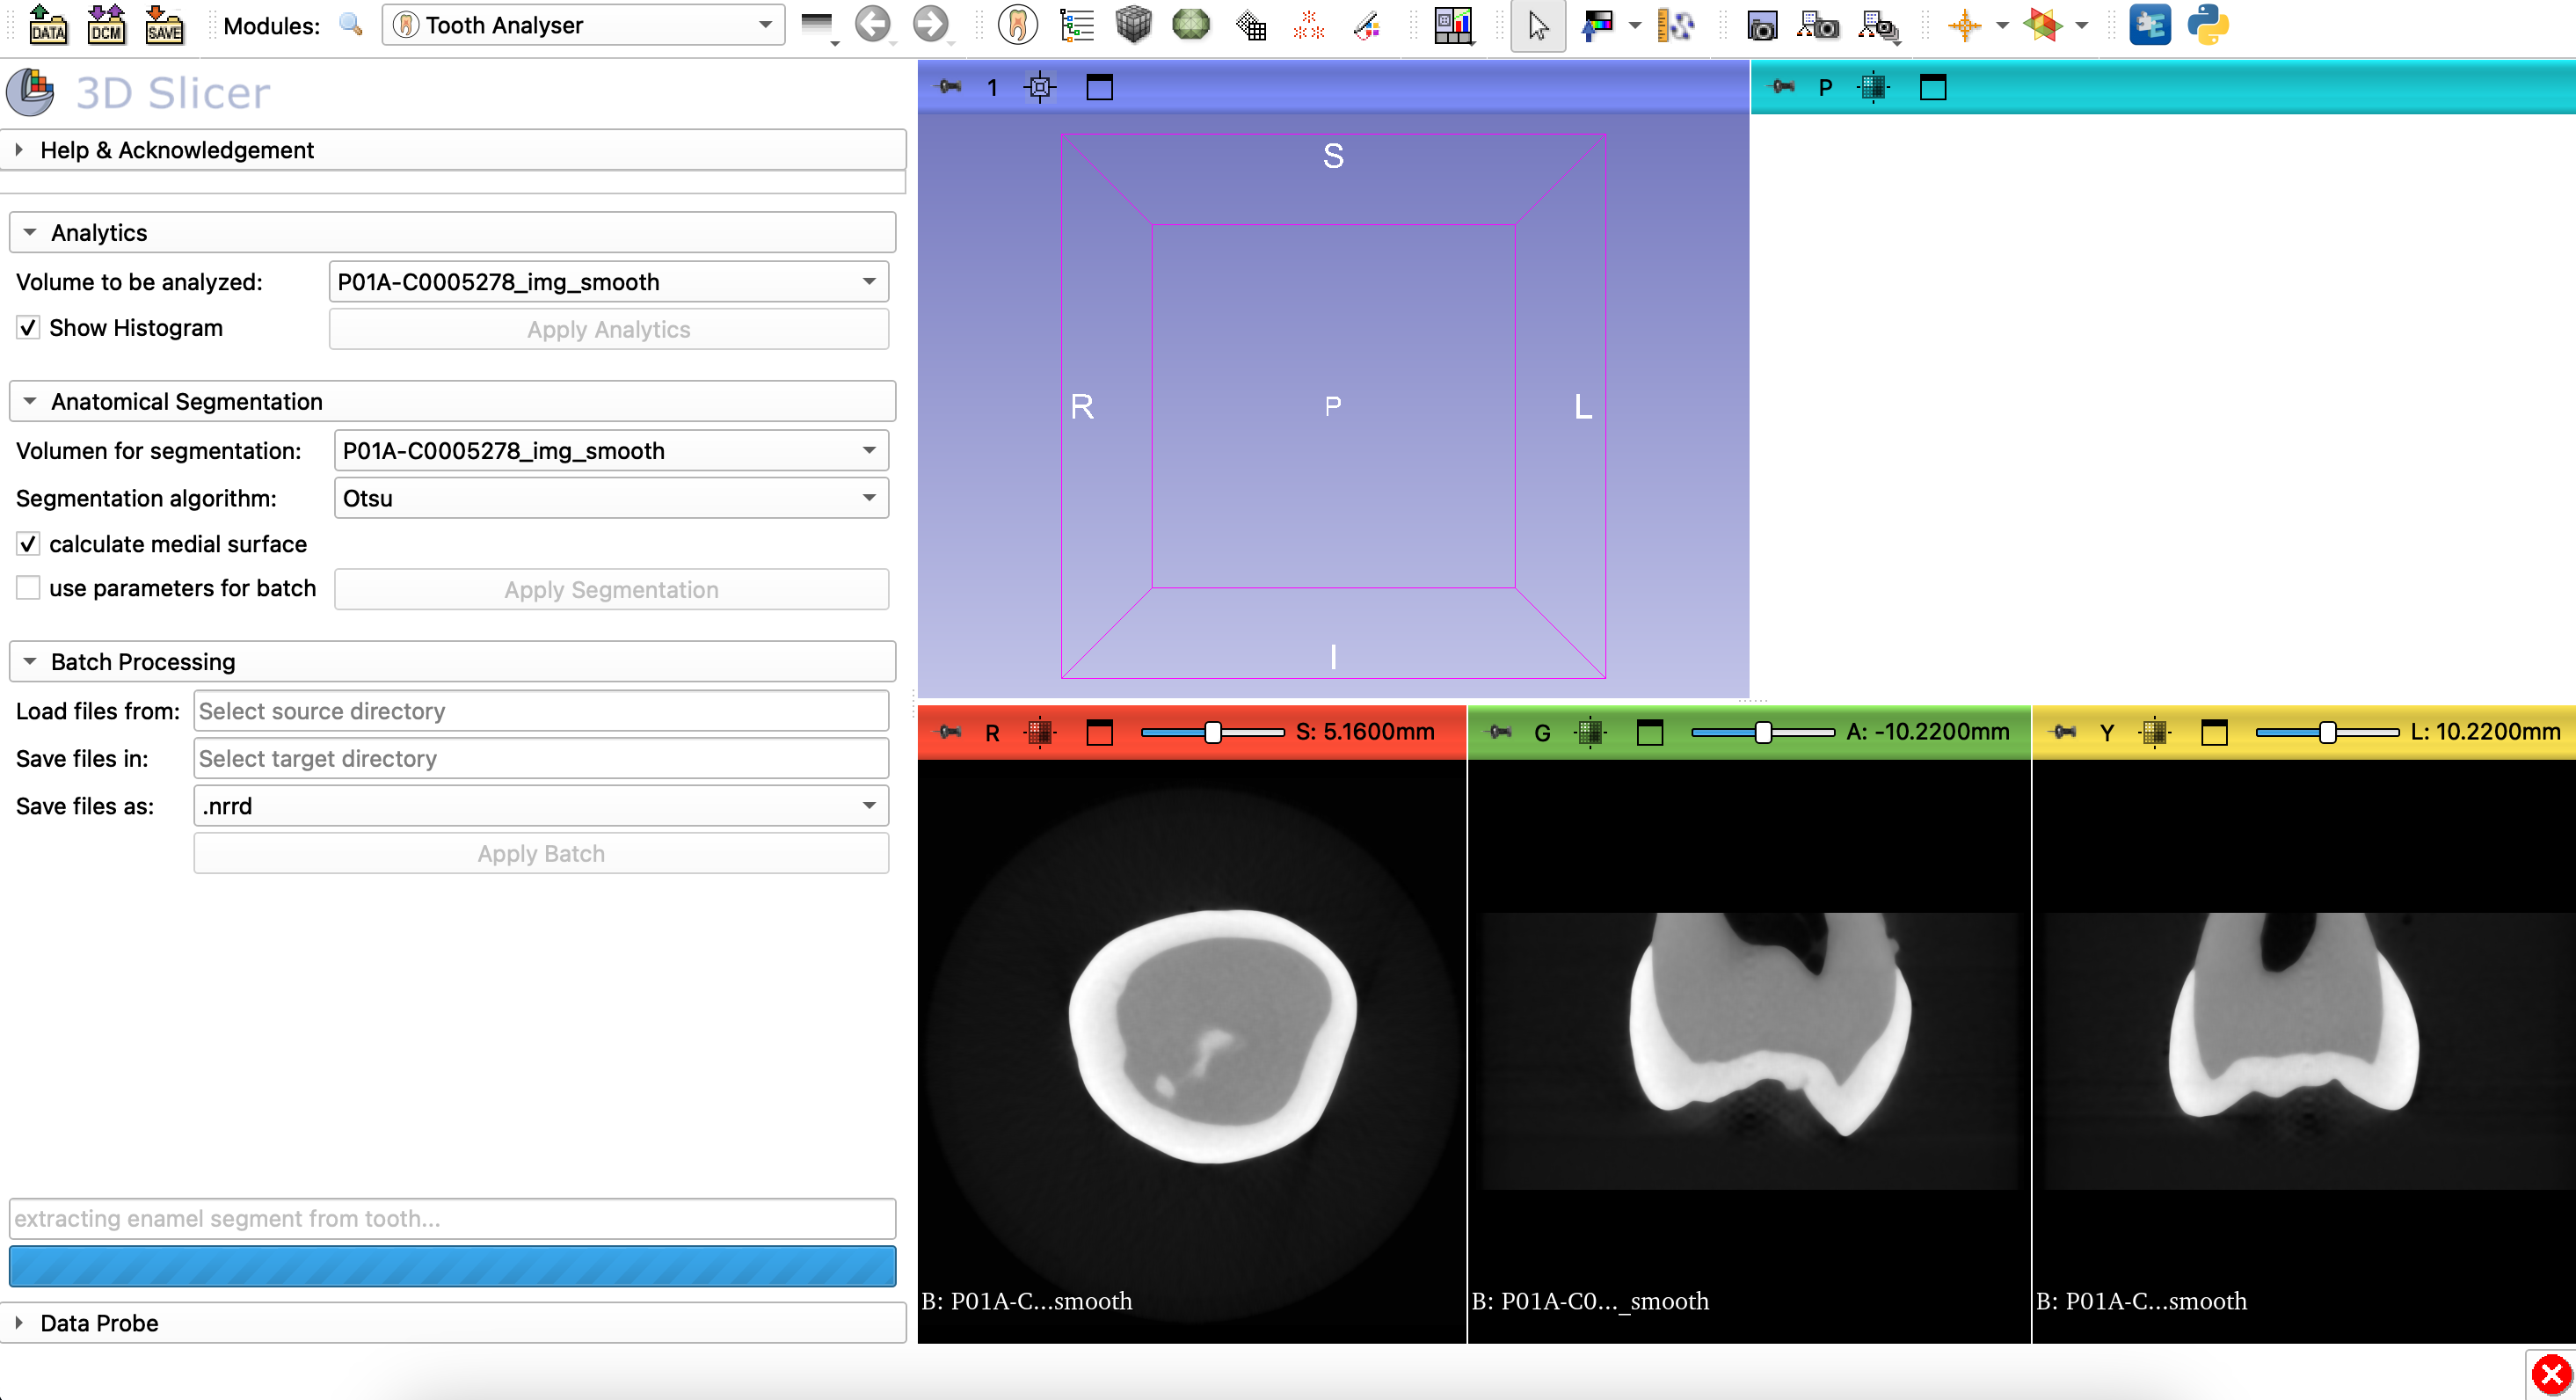
\includegraphics[scale=1, width=\textwidth]{img/processingMode.png}
	\caption{Ansicht des Moduls Tooth Analyser während der Ausführung eines
	Verfahrens}
	\label{fig:processing_mode}
\end{figure}

Mit dem Start eines Verfahrens wechselt der Tooth Analyser automatisch in einen
Prozess Modus. Dieser deaktiviert die Buttons zum Ausführen eines Algorithmus.
Des Weiteren wird am unteren Rand des Moduls eine Fortschrittsanzeige mit
Statusleiste angezeigt, um dem Benutzer mitzuteilen, in welchem Schritt er sich
befindet. Der Cursor ändert innerhalb der Anwendung dann den Modus auf warten.
Hierbei ist zu beachten, dass Slicer selber während der Ausführung nicht bedient
werden kann, da die Ressourcen des Prozesses für den laufenden Algorithmus
verwendet werden. Die Dokumentation von Slicer empfiehlt hier auch kein parallelisieren
der Anwendung, da dies zu \ac{GUI} Fehlern führen würde. Der Benutzer muss also
die Zeit schlichtweg abwarten.

Da neben der reinen Erstellung noch weitere Anforderungen an die Erweiterung
gegeben waren, beschäftigt sich die nächsten Kapitel tiefer mit den softwaretechnischen
Aspekten des Tooth Analyser. Hierzu sollen auch die einzelnen Teilaufgaben, die zu
Beginn definiert wurden, wieder aufgegriffen werden.
% ---------------------------------------------------------------------------------------

\section{Tooth Analyser Bibliothek}
Eine dieser Teilaufgaben beschäftigte sich mit der Integration der anatomischen
Segmentierung welches prototypisch als Python Notebook bereitgestellt wurde. Dieses
Notebook funktioniert, war aber nicht gut strukturiert. So viel es schwer den Überblick
darin zu bewahren und das Verfahren gut nachzuvollziehen. Die gute
Quelltextdokumentation kompensiert dies etwas. Für das von Herrn Hofmann entwickelte
Verfahren wurde demnach ein eigenes Python-Modul erstellt. Somit konnte der
Algorithmus von Aktivitäten in Slicer gut getrennt werden. Das Verfahren selber wurde
gut strukturiert in Funktionen gekapselt, sodass schnell erkannt werden kann, in
welchem Kontext gerade gearbeitet wird. Die einfache Quelltextkommentierung
wurde als Dokumentationsblock an die jeweilige Funktion gehängt. Um die Einordnung
des Moduls für die anatomische Segmentierung besser einordnen zu können, sei die
Projektstruktur hier gezeigt.

\begin{lstlisting}[
    language={python},
    caption={Projektstruktur des Moduls Tooth Analyser mit Fokus auf die ToothAnalyserLib},
    label={lst:projektverzeichnis}]
|-- ToothAnalyser
|   |-- CMakeLists.txt
|   |-- Testing
|   |-- Resources
|   |-- ToothAnalyser.py
|   |-- ToothAnalyserLib
|   |   |-- NewFunction
|   |   |-- AnatomiclasSegmentation
|   |   |   |-- __init__.py
|   |   |   |-- Segmentation.py
|   |   |   |-- isq_to_mhd.py
\end{lstlisting}

Zu sehen ist der Ordner \texttt{ToothAnalyser}, der alle Datei beinhaltet, die
für das Modul relevant sind. Die Datei \texttt{TootAnalyser.py} ist das
Hauptskript und stellt die hier die Anbindung an Slicer dar. Außerdem ist Ordner
\texttt{ToothAnalyserLib} zu finden, der den ganzen externen Quellcode für das Modul
beinhaltet. So auch die anatomische Segmentierung. Kommen in Zukunft weitere Funktionen
dazu, kann diese Bibliothek problemlso um neue Funktionen erweitert werden. Dies
symbolisiert der Ordner \textsl{NewFunktion}. Soll eine Funktion aus dieser Bibliothek
verwendet werden, so kann dies im Modul \texttt{ToothAnalyser.py} einfach über den
folgenden Befehl erfolgen.

\begin{lstlisting}[
    language={python},
    caption={Importieren von Funktionen aus der Bibliothek des Tooth Analyser},
    label={lst:tooth_analyser_lib}]
from ToothAnalyserLib.AnatomicalSegmentation.Segmentation
	import (loadImage, isSmoothed)
\end{lstlisting}

Betrachtet man das Pythonpaket der anatomischen Segmentierung genauer, so fällt auf,
dass es sich in zwei Module teilt. Im Modul \texttt{Segmentation.py} befinden
sich alle Funktionen, die zum Ausführen der Pipeline für die anatomische Segmentierung
notwendig sind. Darüber hinaus finden auch einige Hilfsfunktionen Platz. Das Modul
\texttt{isq\_to\_mhd.py} liefert das Skript, mit dem Dateien im Format \ac{ISQ}
in eine \ac{mhd} Datei umgewandelt werden können. Für die Anwendung im Tooth
Analyser wurde diese Methode leicht modifiziert.

\begin{lstlisting}[
    language={python},
    caption={Modifizierte Methode zum erstellen einer \ac{mhd} Datei aus einem \ac{ISQ} Format},
    label={lst:isq_mhd}]
def isq_to_mhd_as_string(isq_file_name) -> str:
    mhd_param, offset, grey_range = _read_isq_param(isq_file_name)
    mhd_param['ElementDataFile'] = isq_file_name

    # Use a StringIO buffer to construct the MHD content
    mhd_buffer = StringIO()
    for key, value in mhd_param.items():
        mhd_buffer.write(f"{key} = {value}\n")
    return mhd_buffer.getvalue()
\end{lstlisting}

Der Quellcode aus \ref{lst:isq_mhd} zeigt, dass statt einer Abspeicherung auf
der Festplatte ein Pufferspeicher genutzt wird (Zeile acht). Anstatt dann auf die
abgespeicherte Date zu verweisen wird einfach der Pufferspeicher ausgelesen.

Nachdem zu Beginn ein Gesamtüberblick über die Ergebnisse gewonnen wurde und damit
das Modul Tooth Analyser eingeführt wurde, folgen nun die Lösungen der
restlichen Teilaufgaben in Form von Implementierungsdetails.

\pagebreak
% ---------------------------------------------------------------------------------------

\section{Konzeptionen}
\label{sec:konzeptionen} Die ausgearbeiteten Konzeptionen bilden überwiegend die
Ergebnisse der in \ref{sec_zerlegung_in_teilprobleme} beschriebenen Teilaufgaben.
Konkret soll das bedeuten, dass hier konzeptionell gezeigt wird, wie die
softwaretechnischen Aspekte aus den Anforderungen umgesetzt wurden. Hierzu soll zunächst
das Design-Klassendiagramm betrachtet werden, das sich aus dem Domänenmodell in
Abbildung \ref{fig:3d_slicer_domäne} ableiten lässt.

\begin{figure}[h]
	\centering
	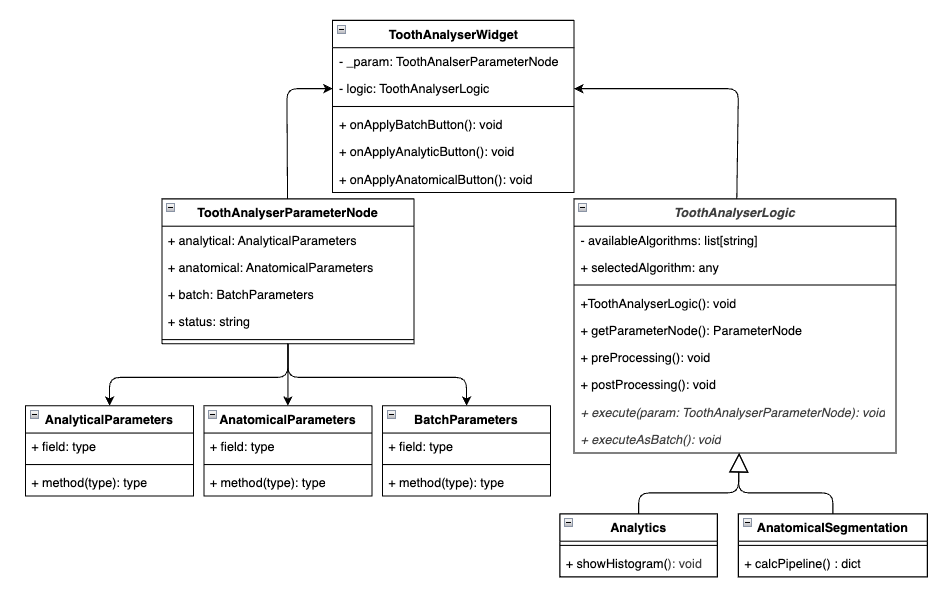
\includegraphics[width=0.9\textwidth]{
		img/tooth_analyser_class_diagram_light.png
	}
	\caption{Ausschnitt aus dem Klassendiagramm für den Tooth Analyser}
	\label{fig:klassendiagramm}
\end{figure}

Wie das Diagramm zeigt, ist die Anwendung über die Klasse \texttt{ToothAnalyserWidget}
in das Kernsystem eingebunden. Sie hält auf der einen Seite alle Parameter der
verschiedenen Funktionen und auf der anderen Seite die dazugehörigen Logiken. Des
Weiteren bildet diese Klasse die gesamt UI des Tooth Analyser ab, was unter
anderem das Laden der \ac{UI} mit einschließt. Die UI des Tooth Analyser wurde
mit der Software QT-Designer erstellt und dann mittels einer Methode in die
Anwendung geladen.

Wie auch schon im Kapitel \ref{sec:tooth_analyser} beschrieben teilt sich die
\ac{UI} auch hier sichtbar in unterschiedliche Teile auf. Betrachtet man nun
Abbildung \ref{fig:klassendiagramm} so fällt auf, das Für jeden Funktionsbereich
eine eigene Parameterklasse erstellt wurde, die dann wiederum in der Klasse
ParameterNode zusammengefasst werden. Dies stellt eine gute Erweiterbarkeit der \ac{UI}
um zusätzliche Parameter sicher. Es wurde an dieser Stelle bewusst keine Generalisierung
verwendet, da Slicer genau diesen konzeptionierten Mechanismus vorsieht. Auf der
anderen Seite der Struktur finden sich die Logikklassen. Die verschiedenen
Logiken die aktuell und zukünftig den Tooth Analyser ausstatten, verwenden alle dieselbe
Schnittstelle, die über die Klasse \texttt{ToothAnalyserLogic} bereitgestellt wird.
Soll also in Zukunft weitere Funktionen hinzukommen, so kann hier einfach eine weitere
Klasse an die Schnittstelle angehängt werden. So entsteht etwas was man in der
Fachliteratur als \textit{Strategy Pattern} bezeichnet \citep[vgl.][S. 99]{siebler2014}.
Der Benutzer der Software wählt also über die verschiedenen Buttons aus, welche
Strategie er gerade nutzen will. Der Tooth Analyser sorgt dann dafür, dass auch
die richtige Funktion geladen wird. Das Feature für den Batch Modus funktioniert
nach einem anderen Schema. Da dieser Modus auch für alle zukünftigen Funktionen
gelten soll, wird dieser nicht als eigene Strategie, sondern direkt in der
Schnittstelle bereitgestellt. So ist sichergestellt, dass eine Implementierung
erfolgen muss, sie jedoch für alle Strategien unterschiedlich sein kann. Um noch
etwas genauer zu zeigen, welche Schritte notwendig sind um den Tooth Analyser mit
weiteren Funktionen auszustatten sei auf Abbildung \ref{fig:klassendiagramm_new}
verwiesen. Hier wird deutlich, welche Klassen und Methoden erstellt werden müssen.

\begin{figure}[h]
	\centering
	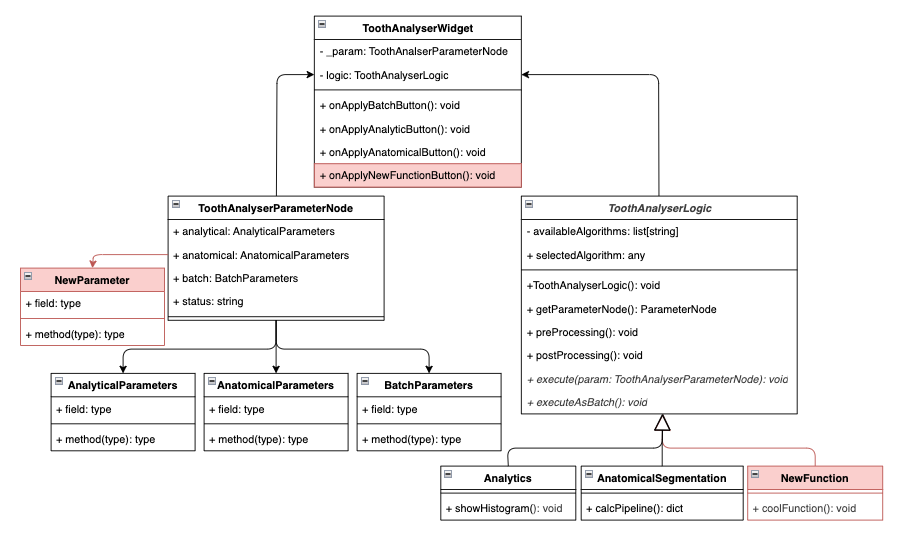
\includegraphics[width=0.9\textwidth]{
		img/tooth_analyser_class_diagram_new.png
	}
	\caption{Hinzufügen neuer Funktionen zum Tooth Analyser}
	\label{fig:klassendiagramm_new}
\end{figure}

Wie bereits zu erkennen ist, signalisieren die roten Elemente die Punkte, an
denen die Funktionalität erweitert werden kann. Die gestrichelte, rote Linie
verdeutlicht nur den Zusammenhang dieser Komponenten und hat keine Auswirkung
auf die Konzeption. Um einen noch genaueren Einblick in die Strukturen zu geben,
geht das nachfolgende Kapitel noch einen Schritt weiter und geht auf konkrete
Implementierungsdetails ein.

\pagebreak
% ---------------------------------------------------------------------------------------

\section{Technische Umsetzung}
\label{sec:technische_umsetzung} Zu Beginn sei gesagt, dass dieses Kapitel nicht
alle Funktionen detailliert beschreibt, sondern sich auf die wichtigsten Funktionen
und Methode des Tooth Analyser beschränkt. Auf Basis des Klassendiagramms aus
Abbildung \ref{fig:klassendiagramm} lässt sich eine grobe Übersicht über die
wichtigsten Klassen gewinnen. Tabelle \ref{tab:methoden_klassen} liefert diese Übersicht.
Die Reihenfolge gibt eine grobe Orientierung bezüglich der Wichtigkeit.

\begin{table}[h]
	\centering
	\begin{tabular}{|c|c|c|}
		\hline
		\textbf{Klassen}             & \textbf{Beschreibung}                              \\
		\hline
		\texttt{ToothAnalyser}       & Klasse für den Abschnitt Hilfe                     \\
		\hline
		\texttt{ToothAnalyserWidget} & Die \ac{UI}-Klasse mit Anbindung an das Kernsystem \\
		\hline
		\texttt{ToothAnalyserLogic}  & Die Logik-Schnittstelle                            \\
		\hline
	\end{tabular}
	\caption{Wichtige Klassen und Methoden im Tooth Analyser}
	\label{tab:methoden_klassen}
\end{table}

Die drei Klassen aus der eben gezeigten Tabelle werden von der Slicer Dokumentation
grob vorgeschrieben, und bilden somit den Kern der Erweiterung. Die Klasse \texttt{ToothAnalyser}
bildet hierbei den Abschnitt \textit{Help and Acknowledgemt}, den jedes Modul
mitbringen muss. Dort stehen alle wichtigen Meta-Informationen über das konkrete
Modul. Der nachfolgende Ausschnitt eines Quelltextes zeigt grob den Aufbau
dieser Klasse.

\begin{lstlisting}[
    language={python},
    caption={Grober Aufbau der Klasse ToothAnalyser nach der Slicer Dokumentation},
    label={lst:3d_slicer_test_class}]
class ToothAnalyser(ScriptedLoadableModule):
    def __init__(self, parent):
	    ScriptedLoadableModule.__init__(self, parent)
	    self.parent.title = _("ExtensionName")
	    self.parent.categories = ["categories"]
	    self.parent.dependencies = ["moduels"]
	    self.parent.contributors = ["author"]
	    self.parent.helpText = _("help")
	    self.parent.acknowledgementText = _("ackn.")
\end{lstlisting}

Direkt in Zeile eins ist zu sehen, dass die Klasse eine Generalisierung der
Klasse \texttt{ScriptedLoadableModule} ist. Über diese Elternklasse wird die
Integration in die Slicer Kernanwendung sichergestellt. Innerhalb des Konstruktors
der Klasse werden unterschiedliche Felder angelegt, welche die verschiedenen
Texte widerspiegeln sollen. Zu Beachten ist noch, dass die Felder die einen
einfachen String erwarten, in einer unscheinbaren Methode \texttt{\_()}
gekapselt sind. Diese Methode ist Teil des Slicer Python Framework und sorgt dafür,
dass automatisch der Kontextname gewechselt wird. Über bekannte Html-Tags können
auch Bilder oder Hyperlinks eingebaut werden, welche auf Screenshots oder
Dokumentationen verweisen.

Die Klasse \texttt{ToothAnalyserWidget} bildet die gesamte Benutzerschnittstelle
der Erweiterung ab und kümmert sich gleichzeitig um das Zusammenspiel zwischen Logik
und Parameter. Hierfür hat die Widget-Klasse Zugriff auf alle Parameter und auf
die Logik-Schnittstelle. Das nachfolgende Listing zeigt einen groben Aufbau der Klasse
\texttt{ToothAnalyserWidget} und deren Felder.

\begin{lstlisting}[
    language={python},
    caption={Grober Aufbau der Widget-Klasse und deren Felder},
    label={lst:create_ui}]
class ToothAnalyserWidget(ScriptedLoadableModuleWidget):
  def __init__(self, parent=None) -> None:
    ScriptedLoadableModuleWidget.__init__(self, parent)
    self.logic = None
    self._param = None
\end{lstlisting}

Wie auch schon die Klasse \texttt{ToothAnalyser} ist auch die Widget-Klasse eine
Kindklasse. Der Konstruktor dieser Klasse wird jedes Mal aufgerufen, wenn der
Benutzer zum ersten Mal nach dem Start von Slicer das Modul aufruft. Neben dem Konstruktoraufruf
der Elternklasse, werden auch die Parameter und die Logik-Schnittstelle
initialisiert. So ergibt sich die Situation, dass die UI die aktuellen
Parametereinstellungen abfragt und sie and die Logik weiterleitet.

Neben der Steuerungsaufgabe erstellt die Widget-Klasse auch die UI aus der .ui Datei.
Da diese unter der Haube ein XML Format aufweist, kann diese einfach in das Modul
hineingeladen werden. Der Quellcode aus ... zeigt dies.

\begin{lstlisting}[
    language={python},
    caption={Laden der \ac{UI} in das Modul ToothAnalyser},
    label={lst:create_ui}]
def createUI(self) -> any:
  uiWidget = slicer.util.loadUI(self.resourcePath("UI/W.ui"))
  self.layout.addWidget(uiWidget)
  self.ui = slicer.util.childWidgetVariables(uiWidget)
  return uiWidget
\end{lstlisting}

Mittels der Bibliothek \texttt{slicer} lässt sich hier die Datei für die \ac{UI}
laden. Diese Datei liegt im Ordner \textit{Resources} sodass der Pfad zu diesem Ordner
mit der Methode \texttt{self.resourcePath()} ausgelesen werden kann. Als Argument
kann dann der Name der Datei angegeben werden. In diesem Fall existiert noch ein
Unterordner mit der entsprechenden Datei (\texttt{"UI/W.ui"}).

Ein weiterer nennenswerter Punkt in der Klasse \texttt{ToothAnalyserWidget} sind
die eventbasierten Methoden. Diese sorgen dafür, dass auf bestimmte Aktionen in
der Anwendung reagiert werden kann. Der Tooth Analyser hat in der Widget-Klasse mehrere
solcher Event-Methoden, die hier genannt werden.

\begin{description}
	\item[\textbf{enter()}] wird immer ausgeführt, wenn der Benutzer das Modul
		öffnet

	\item[\textbf{exit()}] wird immer ausgeführt, wenn der Benutzer ein anderes
		Modul öffnet

	\item[\textbf{onSceneStartCloes()}] wird immer ausgeführt, kurz bevor das
		Modul geschlossen wird

	\item[\textbf{onSceneEndClose()}] wird ausgeführt, nachdem das Modul
		geschlossen wurde

	\item[\textbf{observeParameter()}] wird ausgeführt, wenn der Benutzer
		Änderungen an der \ac{UI} macht
\end{description}

Die Methode \texttt{observerParameter()} ist hierbei sehr interessant und
verdient besondere Beachtung. Die Methode ist eine Beobachtungsmethode, die an
ein Event gekoppelt ist, dass sich \textit{ModifiedEvent} nennt. Dieses Event wird
immer ausgelöst, wenn der Benutzer Änderungen in der Slicer \ac{UI} macht. Dies
umschließt nicht nur das Modul. Wird also solch ein Event gefeuert, so wird die
Methode \texttt{observeParameter()} aufgerufen. Das Listing
\ref{lst:observe_parameter} zeigt diese Methode:

\begin{lstlisting}[
    language={python},
    caption={Methode zum Beobachten von Änderungen in der Benutzerschnittstelle},
    label={lst:observe_parameter}]
def observerParameters(self, caller=None, event=None)->None:
  self.handleApplyBatchButton()
  self.handleApplyAnalyticsButton()
  self.handleApplyAnatomicalButton()
\end{lstlisting}

Die Methode verfügt über die Parameter \texttt{caller} und \texttt{event}.
Mittels diesen Parametern kann der Auslöser des Events und die Art des Events
bestimmt werden. So könnte man verschiedenen Aktionen auf verschiedene Events ausführen.
Innerhalb des Tooth Analyser wird diese Methode genutzt, um die Klick-Logik der Buttons
abzubilden. Die Methoden \texttt{handleApply<...>Button()} steuern jeweils die Sichtbarkeit
der einzelnen Buttons. Immer wenn der Benutzer dann Änderungen an der UI
durchführt, wird die Logik innerhalb dieser Methode aus Listing \ref{lst:observe_parameter}
aktualisiert.

Die letzte der wichtigen Klassen bildet die Logik-Schnittstelle, wie sie in
Tabelle \ref{tab:methoden_klassen} Zeile drei genannt wurde. Diese Schnittstelle
ist der zentrale Punkt aller aktuellen und zukünftigen Logik-Klassen. Jede
Klasse, die einen speziellen Algorithmus implementiert, muss dieses Interface
implementieren. So wird sichergestellt, dass alle Algorithmen nach dem gleichen
Aufbau eingebaut wurden. Dies sorgt für ein einheitliches Vorgehen. Das Listing
\ref{lst:logik_interface} zeigt diese eben beschriebenen Schnittstelle und soll
diese so genauere beleuchten.

\pagebreak

\begin{lstlisting}[
    language={python},
    caption={Die Logik-Schnittstelle des Tooth Analyser},
    label={lst:logik_interface}]
class ToothAnalyserLogic(ScriptedLoadableModuleLogic):
    def __init__(self) -> None:
        ScriptedLoadableModuleLogic.__init__(self)

    def getParameterNode(self) -> ToothAnalyserParameterNode:
        return ToothAnalyserParameterNode(super().getParameterNode())

    def preProcessing(self) -> None:
        """Implement pre processing here"""
        pass

    def postProcessing(self) -> None:
        """Implement post processing here"""
        pass

    def execute(self, param: ToothAnalyserParameterNode)->None:
        """Abstract method"""
        raise NotImplementedError("Please implement this")

    def executeAsBatch(self, param: ToothAnalyserParameterNode)->None:
        """Abstract method"""
        raise NotImplementedError("Please implement this")
\end{lstlisting}

Auch die dritte der wichtigen Klassen erbt von einer übergeordneten Klasse und
verfügt so über deren Funktionen. Die Schnittstelle verfügt über drei Methoden,
die eine Standardimplementierung haben und direkt im Interface implementiert
werden. Die Methode \texttt{getParameterNode()} sorgt dafür, dass alle Parameter
des Moduls zur Verfügung stehen und verwendet werden können. \texttt{preProcessing()}
und \texttt{postProcessing()} sind für eine Vor- und Nachverarbeitung des entsprechenden
Bildes verantwortlich. Die Vorverarbeitung könnte beispielsweise eine
Komprimierung des Bildes beinhalten, wohingegen die Nachbereitung Analysen auf dem
Ergebnis anstoßen könnte. Im Rahmen dieser vorliegenden Arbeit wurden für die
Methoden \texttt{preProcessing()} und \texttt{postProcessing()} keine
Methodenrümpfe gebaut. Eine mögliche zukünftige Implementierung ist im Kapitel \ref{chap:schlussfolgerung}
zu finden. Die beiden noch übrigen Methoden \texttt{execute()} und \texttt{executeAsBatch()}
sind abstrakte Methoden, die eine Implementierung in den jeweiligen Unterklassen
erfordern. Dabei bilden beide Methoden zentrale Punkte. Innerhalb dieser Methoden
soll der entsprechende Algorithmus der Klasse ausgeführt und gestartet werden.
Einmal mit nur einem Bild und anschließender Visualisierung in der Slicer Szene
und einmal als Batch ohne Visualisierung.

\pagebreak

Um den Zusammenhang der Klassen im Tooth Analyser noch besser verstehen zu können
sollen hier jeweils die nötigen Punkte aus den einzelnen Klassen herausgegriffen
werden. Dies verdeutlicht das Zusammenspiel der Methoden um den zugrunde
liegenden Algorithmus zu starten.

\begin{lstlisting}[
    language={python},
    caption={Die Parameter des Tooth Analyser, die als Attribut in der Widget-Klasse liegen.},
    label={lst:observe_parameter}]
@parameterNodeWrapper
class ToothAnalyserParameterNode:
    analytical: AnalyticalParameters
    anatomical: AnatomicalParameters
    batch: Batch
    status: str = ""
\end{lstlisting}

\begin{lstlisting}[
    language={python},
    caption={Starten des Algorithmus durch den Aufruf der \texttt{execut()} Methode in der Widget-Klasse. Die Parameter werden mit übergeben.},
    label={lst:observe_parameter}]
def onApplyAnatomicalButton(self) -> None:
    self.activateComputingMode(True)
    with slicer.util.tryWithErrorDisplay(_("Failed")):
	  try:
	    AnatomicalSegmentationLogic.execute(self._param)
	  except:
	    slicer.util.errorDisplay(_("Error"))
    self.activateComputingMode(False)
\end{lstlisting}

\begin{lstlisting}[
    language={python},
    caption={Ein Ausschnitt der Methode \texttt{execute()}, welche die Pipeline für das Verfahren startet und in der Widget-Klasse durch den Apply-Button aufgerufen wird.},
    label={lst:observe_parameter}]
@classmethod
def execute(cls, param: ToothAnalyserParameterNode) -> None:
    toothDict = cls.calcPipeline(
	    sourcePath=sourcePath,
	    calcMidSurface=param.anatomical.calcMidSurface,
	    param=param,)
\end{lstlisting}

Die Parameter, die im Parameter Knoten gespeichert werden liegen wie bereits
beschrieben als Attribut und der Klasse \texttt{ToothAnalyserWidget}. Wenn ein
Button zum Ausführen der entsprechenden Logik gedrückt wird, wird die Methode \texttt{execute()}
ausgeführt und alle Parameter als Argument mit übergeben. So ist innerhalb der Ausführung
ein voller Zugriff auf die Parameter möglich.

Nach der konkreten Umsetzung der Erweiterung kann Schritt für Schritt mit der Evaluation
der Ergebnisse begonnen werden. Ein wichtiger Teil sind die Testergebnisse

\pagebreak
% ---------------------------------------------------------------------------------------

\section{Evaluierung}
\label{subsec:evaluierung} Neben der Implementierung der Features wurden auch
diverse Tests durchgeführt, die eine Bewertung der Ergebnisse möglich machen.
Hierzu wurden Softwaretests, Benutzertests und Messungen durchgeführt. Dieses
Kapitel beschäftigt sich mit der Testauswertung der verschiedenen Testfälle. Begonnen
wird mit einer Analyse der Softwaretests, gefolgt von Laufzeitmessungen. Abschließend
werden die Anwendungsfälle des Tooth Analyser näher beleuchtet und auf die Limitierungen
der Anwendung eingegangen.

\subsection{Softwaretests}
\label{subsec:softwaretests} Betrachtet man die Dokumentation von Slicer genauer,
so fällt auf, dass dies eine recht starre Struktur für die Implementierung von Tests
vorgibt. Dabei ist jedoch nicht festgelegt, welche Art von Tests verwendet werden
soll. Im Rahmen des Tooth Analyser wurden hier ausschließlich Unittest
implementiert, welche die einzelnen Einheiten und Funktionen im Tooth Analyser abdecken.
Der grobe Testaufbau sei hier gezeigt.

\begin{lstlisting}[
    language={python},
    caption={Ausschnitt der Testklasse zum ausführen der Unittests},
    label={lst:observe_parameter}]
class ToothAnalyserTest(ScriptedLoadableModuleTest):
    def setUp(self):
	    slicer.mrmlScene.Clear()
	    self.loadSampleData()

    def runTest(self):
	    self.setUp()
	    self.testIsSmoothed()
	    # add more tests here...

    def testIsSmoothed(self):
	    from ToothAnalyserLib.AnatomicalSegmentation.Segmentation import isSmoothed
	    sampleDate = self.getSampleDataAsITK()
 	    result = isSmoothed(sampleDate)
	    self.assertFalse(result)
	    self.delayDisplay("Test 1 passed")
\end{lstlisting}

Wie gleich zu erkennen ist, wurden alle Softwaretests in der Klasse \texttt{ToothAnalyserTest}
gekapselt. Diese ist wie auch bei einigen anderen Klassen eine generalisierte
Klasse der \texttt{ScriptedLoadableModuleTest}. Der grundsätzliche Aufbau der
Testklasse ist simpel gehalten. Es gibt eine Methode \texttt{setup()} in der die
Testumgebung bereitgestellt wird und eine Methode \texttt{runTest()} in der die einzelnen
Testfälle ausgeführt werden. Betrachtet man die konkrete Testmethode \texttt{testIsSmoothed()}
genauer, so fällt die Methode \texttt{getSampleDataAsITK()} auf, die hier kurz
thematisiert werden soll. Viele der geschriebenen Methoden und Funktionen benötigen
für einen guten Test ein konkretes Bild. Hierfür stellt der Tooth Analyser
Beispielbilder zur Verfügung, mit denen die Tests ausgeführt werden können. Da
diese Bilder eine ausgeprägte Größe haben (ca. 500MB) wurden diese in einem separaten
Repository bereitgestellt. So müssen nicht erst einige \ac{GB} an Bildern heruntergeladen
werden, wenn das Modul installiert werden soll. Die Bilder werden erst dann heruntergeladen,
wenn sie benötigt werden. Um dieses Herunterladen zu ermöglichen, werden die
Bilder beim Starten des Moduls erstmals in Slicer registriert, sodass sie dann im
Modul \texttt{sampleData} zur Verfügung stehen. Damit ist nicht nur gewährleistet,
dass zukünftige Entwickler Tests ausführen könne, es kann so auch Benutzern Beispielbilder
bereitgestellt werden, um erste Efahrungen mit dem Tool zu machen. Die Abbildung
\ref{fig:sample_data} zeigt das Modul \texttt{SampleData} mit besonderem
Augenmerk auf das Bild \textit{ToothCT}.

\begin{figure}[h]
	\centering
	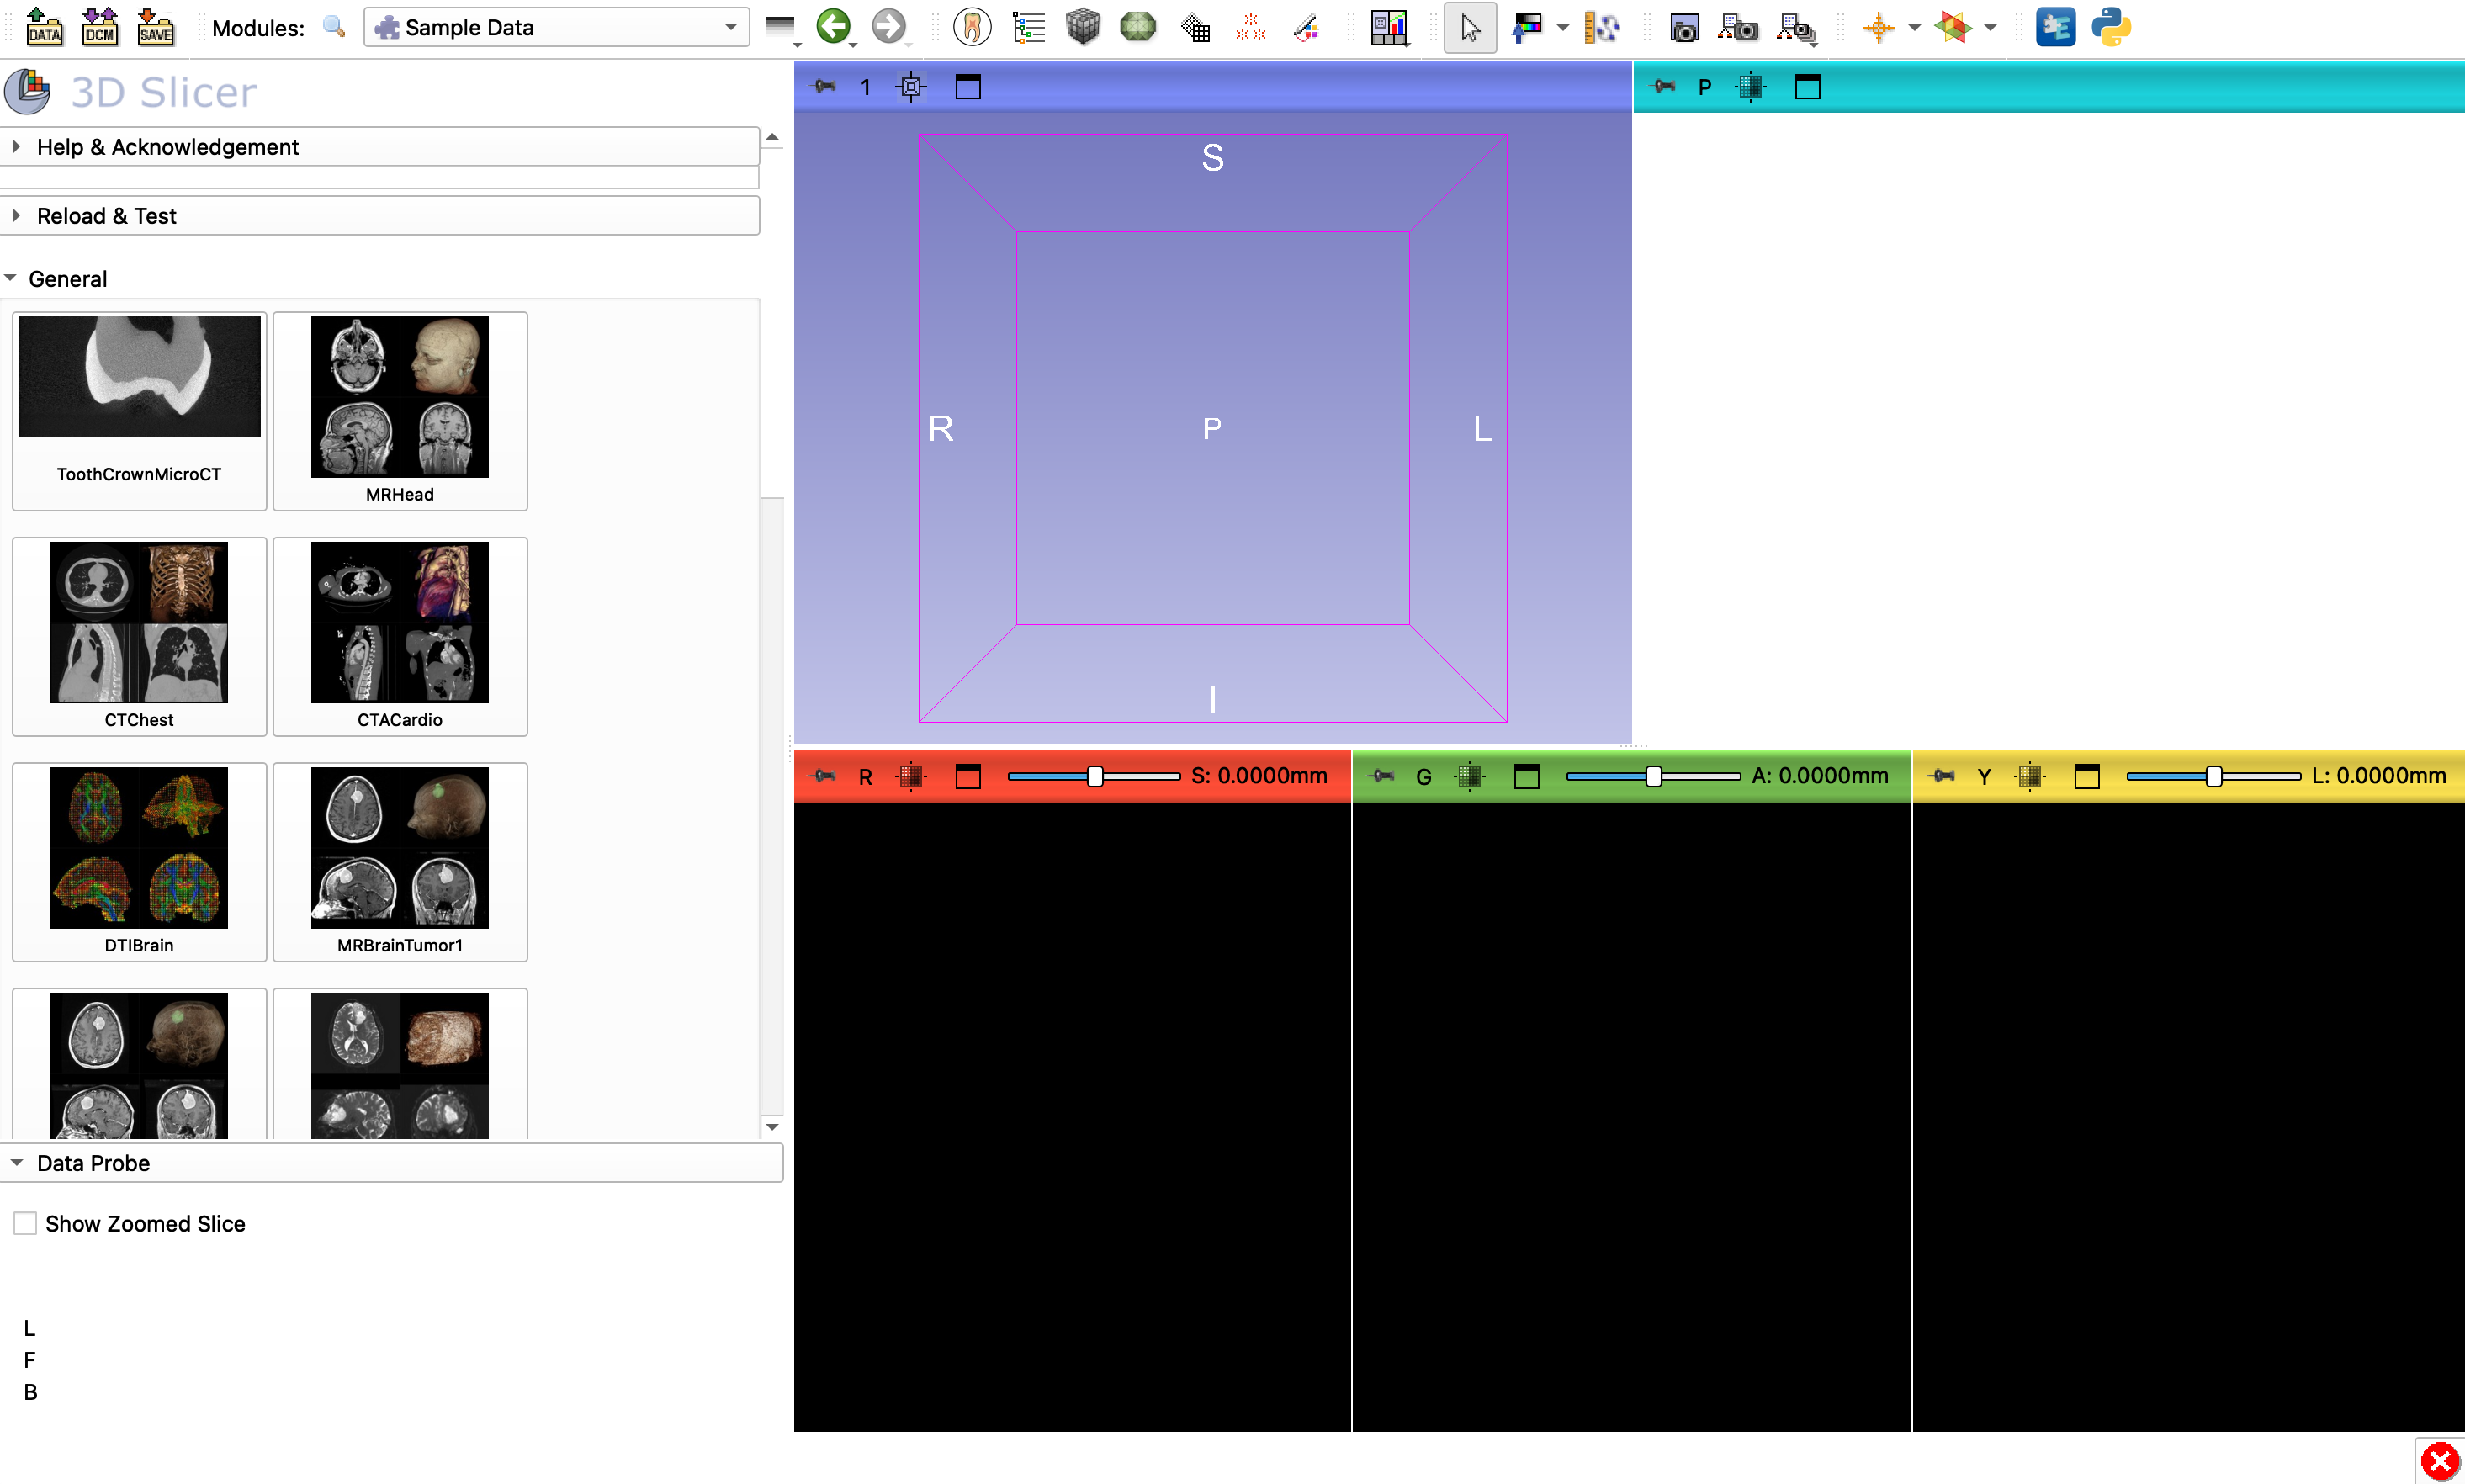
\includegraphics[width=1\textwidth]{img/sampleData.png}
	\caption{Ausschnitt des Moduls SampleData in 3D Slicer}
	\label{fig:sample_data}
\end{figure}

Ein Testfall der vielen soll hier Beispielhaft genauer betrachtet werden. Hierbei
geht es um den Test der Funktion \texttt{smoothImage()}. Diese Nimmt ein Bild und
führt eine Glättung durch. Um solch eine Funktion zu testen, bedarf es etwas mehr
als ein simpler Unittest, jedoch liefert der fertige Test eine gute Lösung um
den gesamten Umfang der Methode zu Testen. Vergleicht man ein verrauschtes Bild mit
einem geglättetes, dann unterschieden sie sich bis auf die visuelle Darstellung
auch in der Streuung der Pixelwerte. So kann mittels der Standardabweichung kontrolliert
werden, ob das Bild nach einer Filterung eine kleinere Standardabweichung hat
als vor dem Bild. Ist dies der Fall, so kann von einer erfolgreichen Filterung
ausgegangen werden. Die konkrete Implementierung eines solchen Tests liefert der
Quellcode \ref{lst:test_smooth_image}.

\begin{lstlisting}[
    language={python},
    caption={Implementierung eines Tests zum überprüfen einer Funktion},
    label={lst:test_smooth_image}]
def testSmoothImage(self):
    from ToothAnalyserLib.AnatomicalSegmentation.Segmentation import smoothImage
   
    data = self.getSampleDataAsITK()
    dataFiltered = smoothImage(data)
    dataStdDev = np.std(sitk.GetArrayFromImage(data))
    dataFilteredStdDev = np.std(sitk.GetArrayFromImage(dataFiltered))
    self.assertTrue(dataFilteredStdDev < dataStdDev)
    self.delayDisplay("Test 1 passed")
\end{lstlisting}

Im ersten Schritt wird ein Beispielbild geladen und in ein \ac{ITK} Format umgewandelt.
Anschließend folgt die Glättung des Bildes. Ist diese Glättung fertig, so können
die Streuungen der beiden Bilder verglichen werden.

Betrachtet man alle Softwaretests, so lässt sich sagen, dass viele und die
wichtigsten Methoden getestet wurde. Jedoch wurden nicht alle Methoden und Funktionen
getestet. Viele bilden eine sehr konkrete Lösung, die nicht einfach zu testen ist
und deshalb einiges an Entwicklungszeit beanspruchen. Eine ebenso gute Aussage
lässt sich anhand der Laufzeit des Moduls treffen. Hierzu wurde die Performance des
Tooth Analyser genauer unter die Lupe genommen.

\pagebreak
% ---------------------------------------------------------------------------------------

\subsection{Performance}
Die Performance des Systems war nie ein wichtiges Kriterium und stand deshalb zu
keiner Zeit im Fokus dieser Arbeit. Dennoch ergaben sich interessante Ergebnisse,
die hier kurz erläutert werden sollen. Unter der Performance versteht dieses Kapitel
das konkrete Laufzeitverhalten der Anwendung also jene Zeit die zwischen Start und
Ende vergeht. Grundsätzlich lässt sich dazu sagen, dass die Laufzeit bei der Bearbeitung
von 3D micro CT Aufnahmen sehr stark vom Type des Bildes abhängt. So kommt es
beispielsweise darauf an, wie groß das Bild ist, oder ob es bereits eine
Filterung erfahren hat. Bei der Verarbeitung der micro CT Bilder aus dem Klinikum
für Zahnerhaltung wurde eine konkrete Messung durchgeführt, die hier in
Abbildung \ref{fig:laufzeit} gezeigt wird.

\textbf{Vorbedingungen:}
\begin{itemize}
	\item 16 bit sigend integer

	\item Type .ISQ

	\item Mit Filterung

	\item Mit Berechnung der medial Flächen
\end{itemize}

\begin{figure}[h]
	\centering
	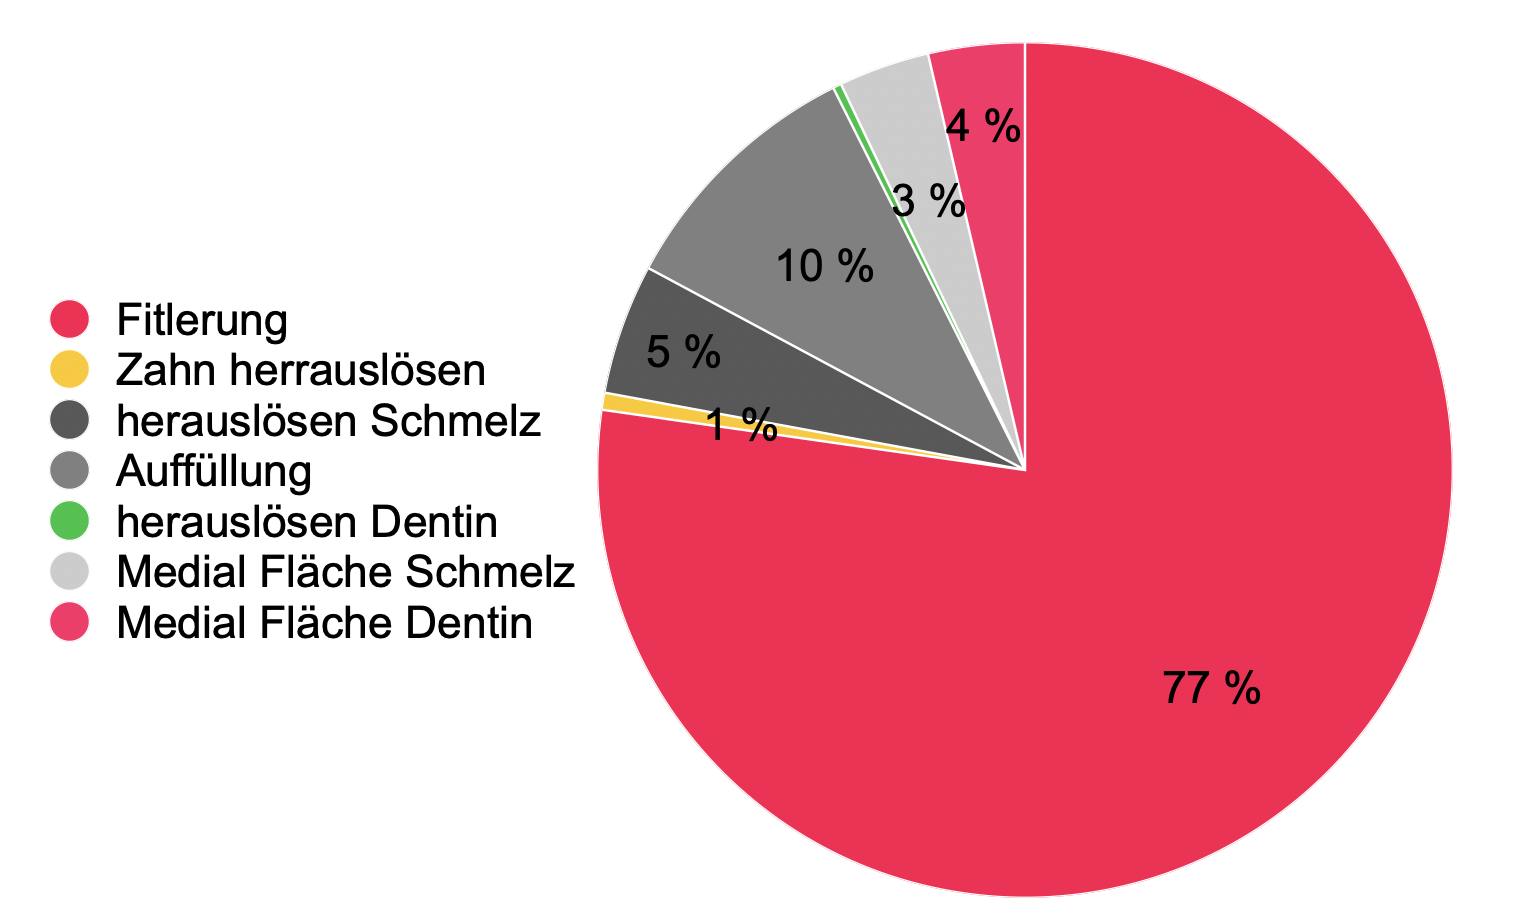
\includegraphics[width=0.8\textwidth]{img/laufzeit_diagramm.png}
	\caption{Verteilung der Laufzeit über den gesamten Bearbeitungszeitraum. 100\%
	entsprechen 16:27 Minuten}
	\label{fig:laufzeit}
\end{figure}

Zu sehen ist, dass unter diesen Bedingungen die Bearbeitung eines einzelnen
Bildes ca. 17 Minuten beansprucht. Dabei fallen über drei Viertel der Zeit auf
die Filterung zurück. Der Bereich Auffüllung beinhaltet ebenfalls eine Filterung
der einzelnen Segmente, weswegen dieser den zweitgrößten Teil ausmacht. Ein Weiterer
wesentlichen Teil stellen die beiden medialen Flächen dar. Um dieser doch
enormen Laufzeit etwas entgegen zu Wirken wurden zwei Mechanismen implementiert.
Das Verfahren kann einerseits erkennen, ob ein Bild bereits gefiltert wurde und
andererseits die medialen Flächen optional berechnen. So kommt es das sich ein \textit{Best
Case} ergibt der grob nur noch ein Viertel der Zeit benötigt. Dieser \textit{Best
Case} tritt ein, wenn ein Bild in den Algorithmus gegeben wird, das bereits
gefiltert wurde und keine medialen Flächen erfordert.

Überträgt man das Laufzeitverhalten eines einzelnen Bildes auf die Bearbeitung
der Bilder in einem Batch Prozess so lässt sich die Laufzeit mit der Anzahl der
zu bearbeitenden Bilder steigend linear ausdrücken. Das Diagramm aus \ref{fig:laufzeit_batch}
zeigt dies.

\begin{figure}[h]
	\centering
	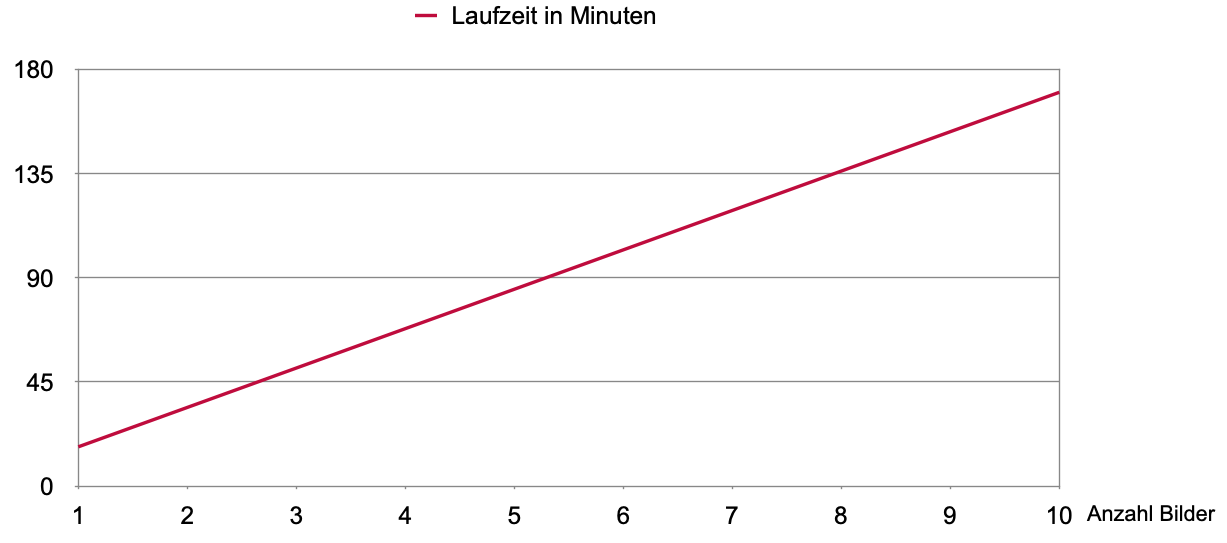
\includegraphics[width=1\textwidth]{img/runtimeBatch.png}
	\caption{Konstruktion des Laufzeitverhaltens bei einer Bearbeitung mehrere
	Bilder}
	\label{fig:laufzeit_batch}
\end{figure}

Wie zu sehen ist, ist die Laufzeit eines Batch Prozesses maßgeblich davon geprägt,
wie lange ein einzelnes Bild benötigt. Ist die Zeit eines einzelnen Bildes bekannt,
so lässt sich gut prognostizieren, wie lange eine Verarbeitung von $n$ vielen Bildern
dauert. Wie bereits angedeutet, hängt die Zeit eines einzelnen Bilds von vielen Faktoren
ab. In diesem Fall würde die Bearbeitung von zehn Bilder etwa 170 Minuten
beanspruchen. Dies entspricht zwei Stunden und 50 Minuten.

Im Rahmen eines kleinen Stresstests wurden 103 CT Aufnahmen aus dem Tooth Analyser
heraus in einem Batch Prozess gestartet. Hierzu wurde ein Server der \ac{LMU} genutzt,
der über große Ressourcen verfügt. Die Bearbeitung eines Bildes benötigt hier etwa
neun Minuten. Befolgt man die Verteilung aus der Abbildung
\ref{fig:laufzeit_batch}, so lässt sich eine Zeit von 15 Stunden und 27 Minuten prognostizieren.
Das Resultat dieses Tests zeigt, das in etwa auch diese Zeit benötigt wurde.
Viel wichtiger ist jedoch, dass hierbei alle Bilder erfolgreich anatomisch segmentiert
werden konnten.

Nichtsdestotrotz bleibt die Anwendung trotz ihrer doch hohen Laufzeit ein enormes
Zeitersparnis für die praktizierenden Ärzte. Laut Dr. Elias Walter würde eine händische
Segmentierung ca. 20 Minuten aktive Arbeit bedeute. Diese Arbeit kann der Tooth Analyser
deutlich reduzieren, indem kein aktives Arbeiten erfordert, sondern im Hintergrund
läuft. Für welche Anwendungsfälle der Tooth Analyser genau eingesetzt werden
kann, darüber berichtet das Kapitel Anwendungsszenarien
% ---------------------------------------------------------------------------------------

\subsection{Anwendungsszenarien}
In erster Linie bietet der Tooth Analyser eine Visualisierungshilfe, die für Ärzte
unterstützend wirken soll. Wie auch von Slicer empfohlen wird dieses Modul von
den Ärzten rein zur Forschung eingesetzt. Mit den Tooth Analyser lässt sich mittels
einer micro CT-Aufnahme ein 3D Modell des Zahnes erstellen. Man spricht hier von
einer Rekonstruktion des Zahnes. Durch die Segmentierung erlaubt dieser rekonstruierte
Zahn auch eine Segmentbetrachtung von Dentin und Schmelz. Die Abbildungen
\ref{fig:3d_view} und \ref{fig:3d_view_dentin} zeigt diese Rekonstruktion
genauer.

\begin{minipage}{0.45\textwidth}
	\centering
	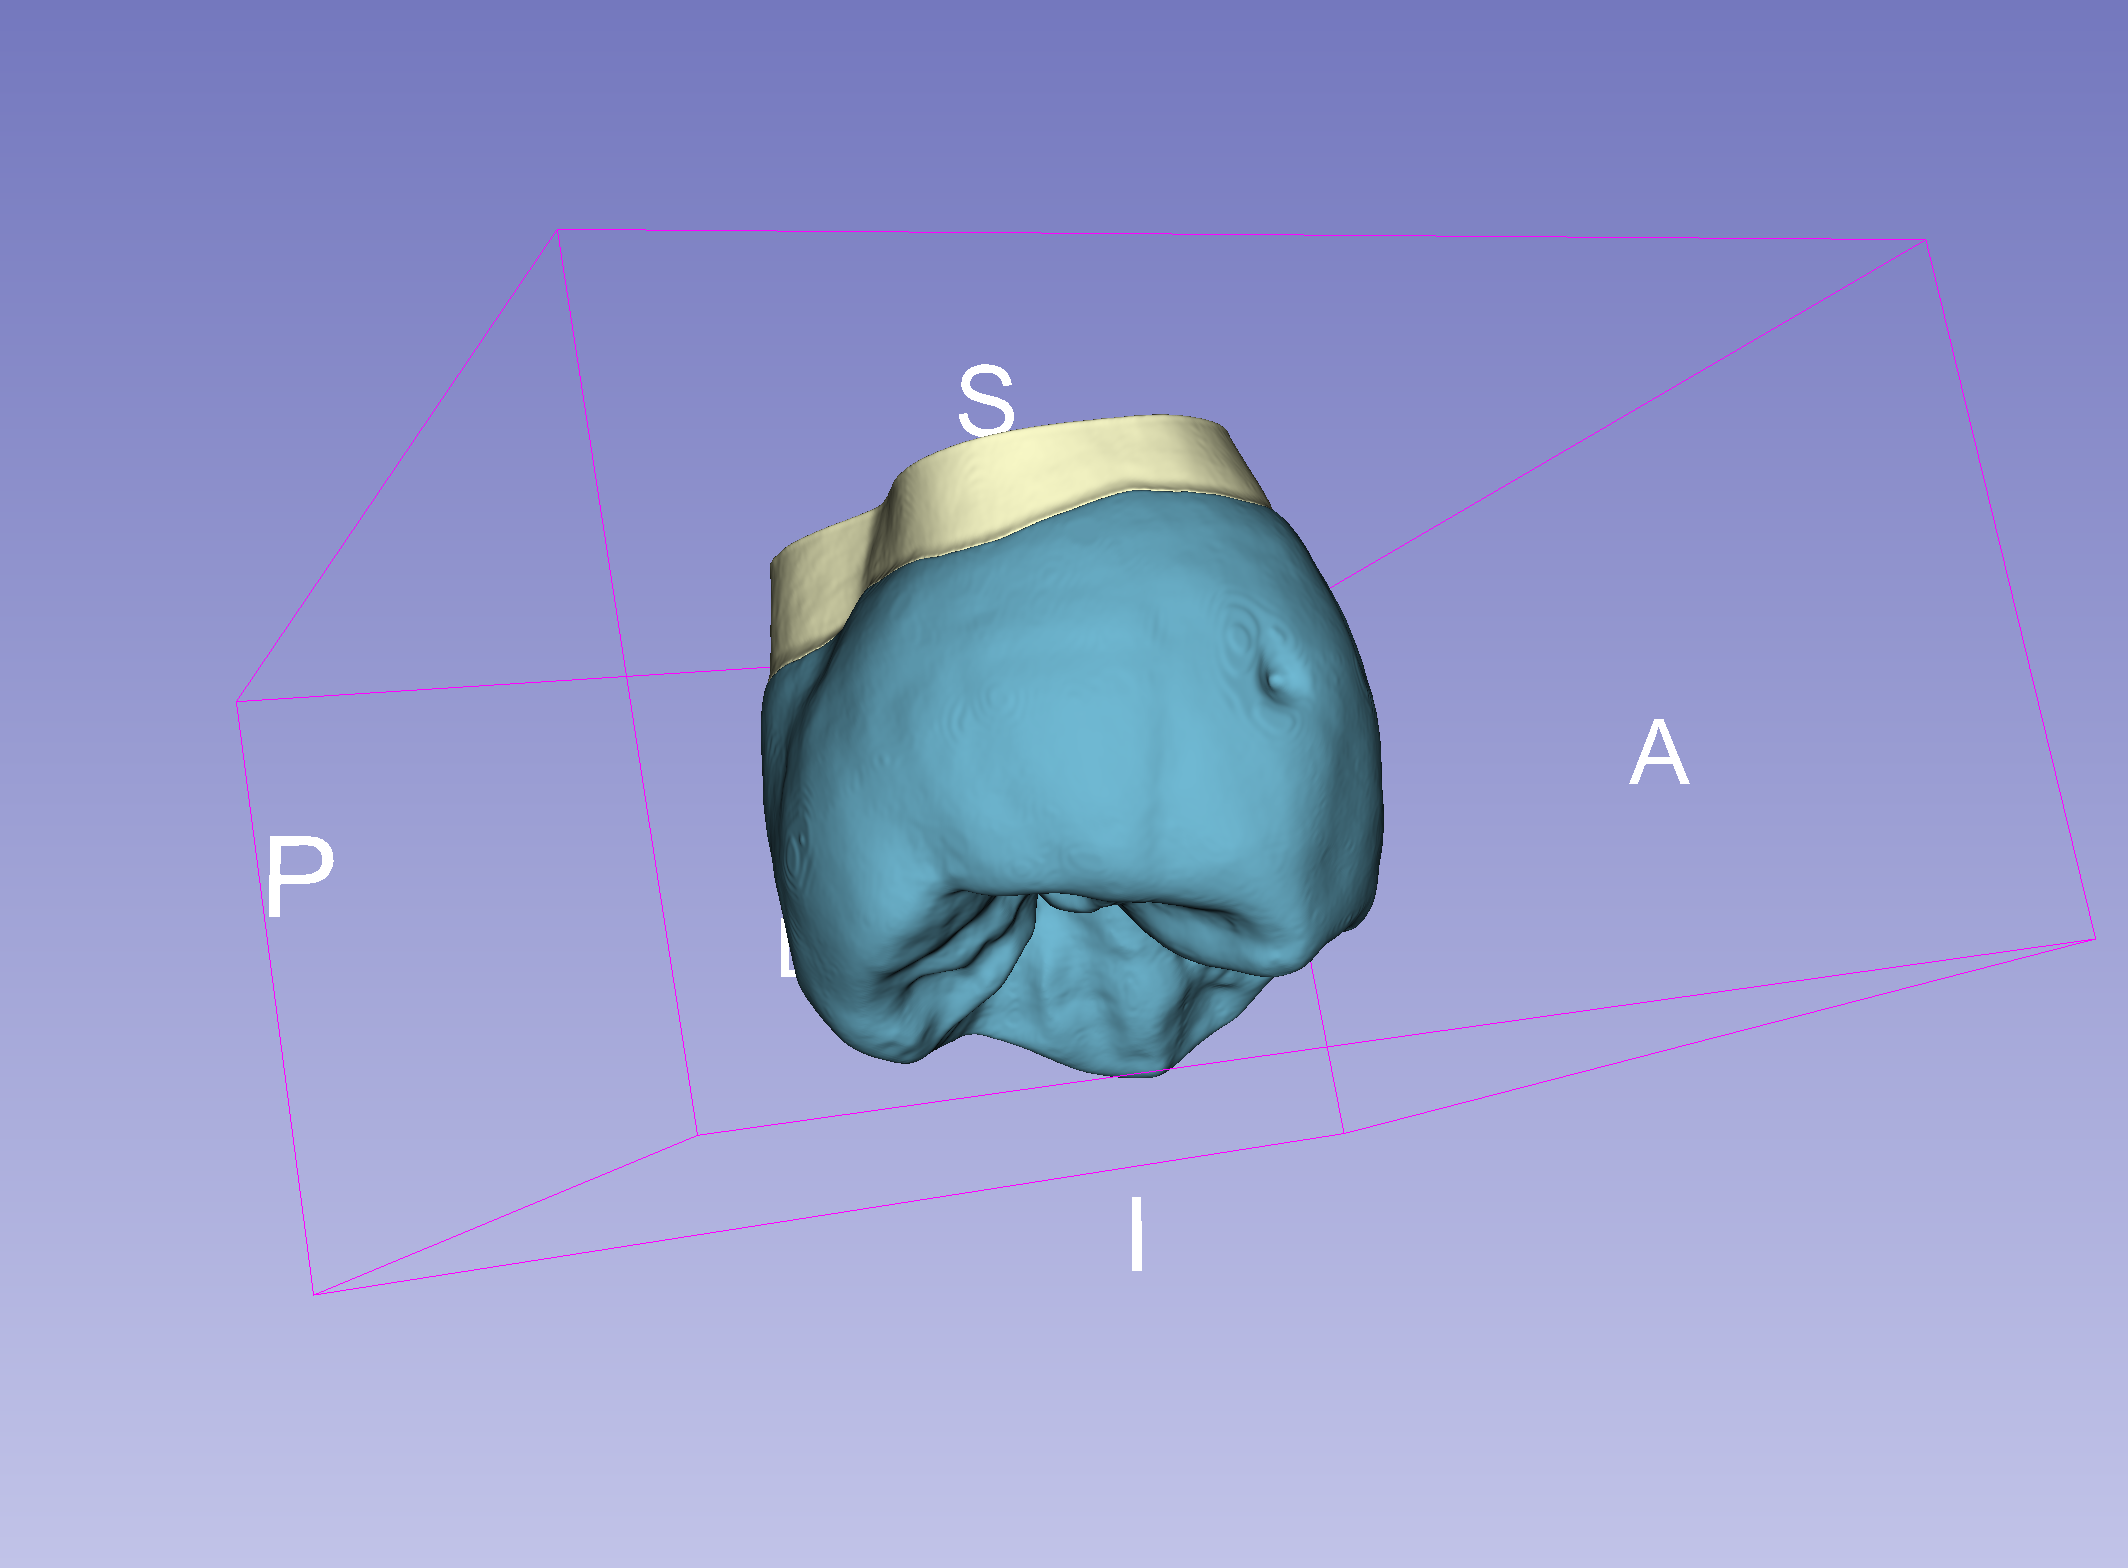
\includegraphics[scale=0.2, width=\textwidth]{img/3dView.png}
	\captionof{figure}{Rekonstruktion eines Zahns aus einer CT-Aufnahme mittels der Erweiterung Tooth Analyser.}
	\label{fig:3d_view}
\end{minipage}
\hfill
\begin{minipage}{0.45\textwidth}
	\centering
	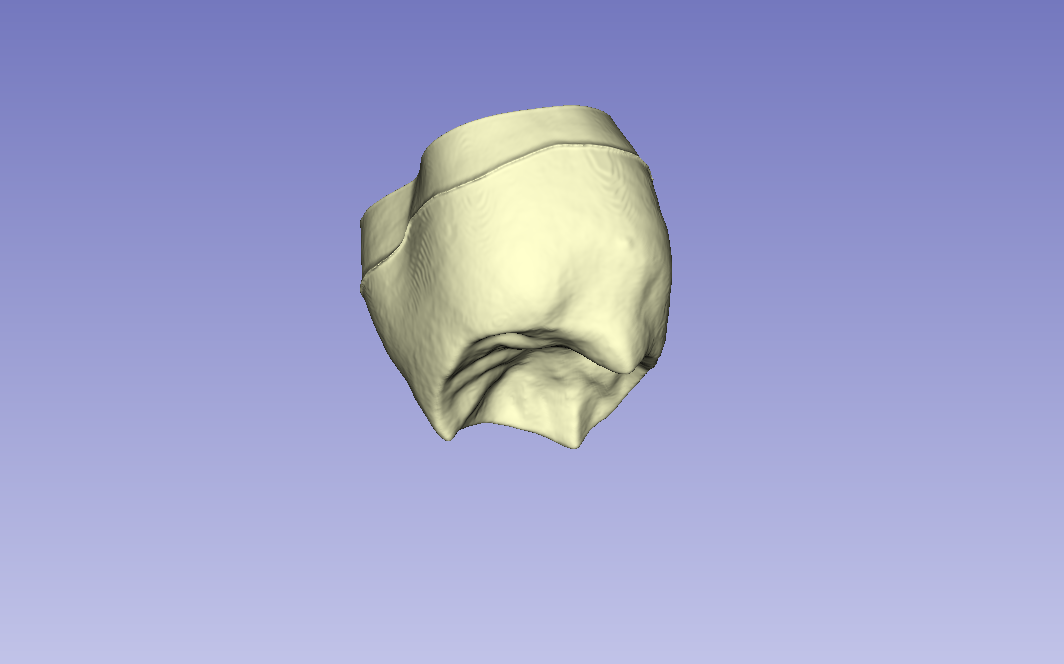
\includegraphics[scale=0.2, width=\textwidth]{img/3dViewDentin.png}
	\captionof{figure}{Segmentbetrachtung eines rekonstruierten Zahns auf Basis einer CT-Aufnahme.}
	\label{fig:3d_view_dentin}
\end{minipage}

Das Betrachten der einzelnen Segmente wie sie in Abbildung \ref{fig:3d_view_dentin}
gezeigt wird, erfolgt nicht in der Erweiterung Tooth Analyser. Hierzu wird auf das
Modul \textit{Data} verwiesen, das eine hierarchische Darstellung aller Daten in
der Szene liefert. Über die Sichtbarkeitseinstellungen der einzelnen
Datenelemente können dann die Segmente sichtbar oder unsichtbar geschaltet
werden. Einen weiteren Fall, indem die Anwendung unterstützen kann, ist die Klassifizierung
von Karies. Die Abbildung \ref{fig:classification} zeigt diesen Fall.

\begin{minipage}{0.45\textwidth}
	Hierfür sind die medialen Flächen der einzelnen Segmente nötig. Diese sind im
	Bild als rote und grüne Linie sichtbar, verteilen sich aber über das ganze 3D Bild,
	was daraus eine Fläche macht. Legt man nun diese Flächen über das originale Bild,
	so lässt sich mittels dieser Linie der Karies auf einem CT gut klassifizieren.
	Diese besagten Linien bilden dann die Grenzen. Ragt der Karies über diese
	mediale Fläche hinaus hat er bereits einen sehr ausgeprägten Zustand und wird
	anders eingeordnet als ein Karies, der die mediale Fläche noch nicht überschritten
	hat.
\end{minipage}
\hfill
\begin{minipage}{0.45\textwidth}
	\centering
	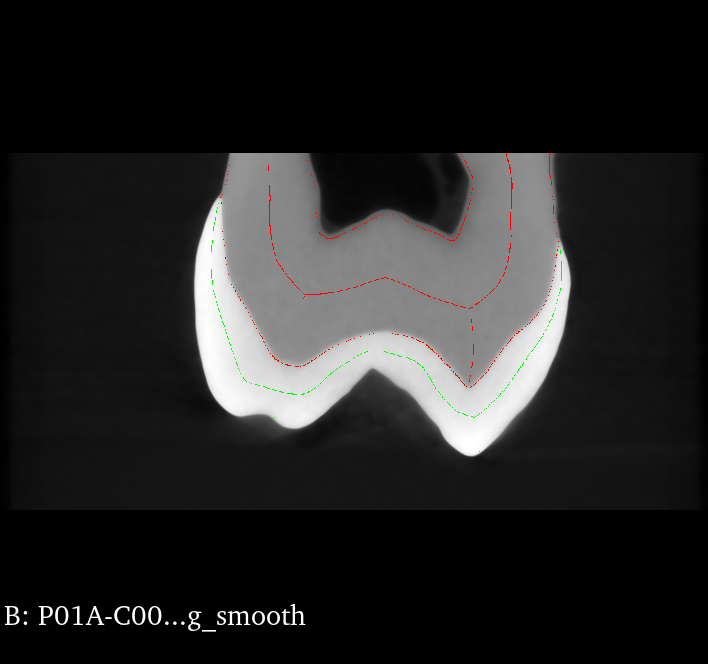
\includegraphics[scale=0.2, width=\textwidth]{img/classification.png}
	\captionof{figure}{Klassifizierung von Karies mittels der medialen Flächen.} \label{fig:classification}
\end{minipage}

Da durch die Klinik für Zahnerhaltung nur CT-Bilder von Zahnkronen bereitgestellt
wurden, wurde der Tooth Analyser auch nur mittels dieser Aufnahmen getestet. Durch
einige Benutzertests in der Klinik zeigte sich aber, dass auch die Segmentierung
eines ganzen Zahns möglich ist. Selbst bei einer komplexeren Wurzel. Jedoch
bleibt es nicht aus, dass der Tooth Analyser auch Einschränkungen mitbringt und so
auch die Verwendung dieses Moduls limitiert.
% ---------------------------------------------------------------------------------------

\subsection{Limitierungen}
\label{sec:limitierungen} Dieses Kapitel soll alle Punkte transparent aufdecken,
die im Modul Tooth Analyser noch Probleme machen, oder gar nicht erst umgesetzt wurden.
Der limitierende Faktor in der Erweiterung ist das eingeschränkte Format der
Bilder. Es können innerhalb dieser Erweiterung nur Bilder verarbeitet werden,
die das Format \ac{Int16} haben. Der Grund hierfür liegt in der Implementierung
des Algorithmus. Die anatomische Segmentierung wurde speziell für die CT-Aufnahmen
im \ac{ISQ} Typ entwickelt. Aus diesem Grund wurden die Schwellwerte und Parameter
für dieses Verfahren fest codiert. Führt man dennoch die Segmentierung mit einem
Bild im Format \ac{8UInt} durch, so stellt man fest, dass der Algorithmus zwar ein
Ergebnis generiert, dieses aber nicht brauchbar ist. Die Abbildung \ref{fig:3d_error}
zeigt ein solches falsche Ergebnis.

\begin{figure}[h]
	\centering
	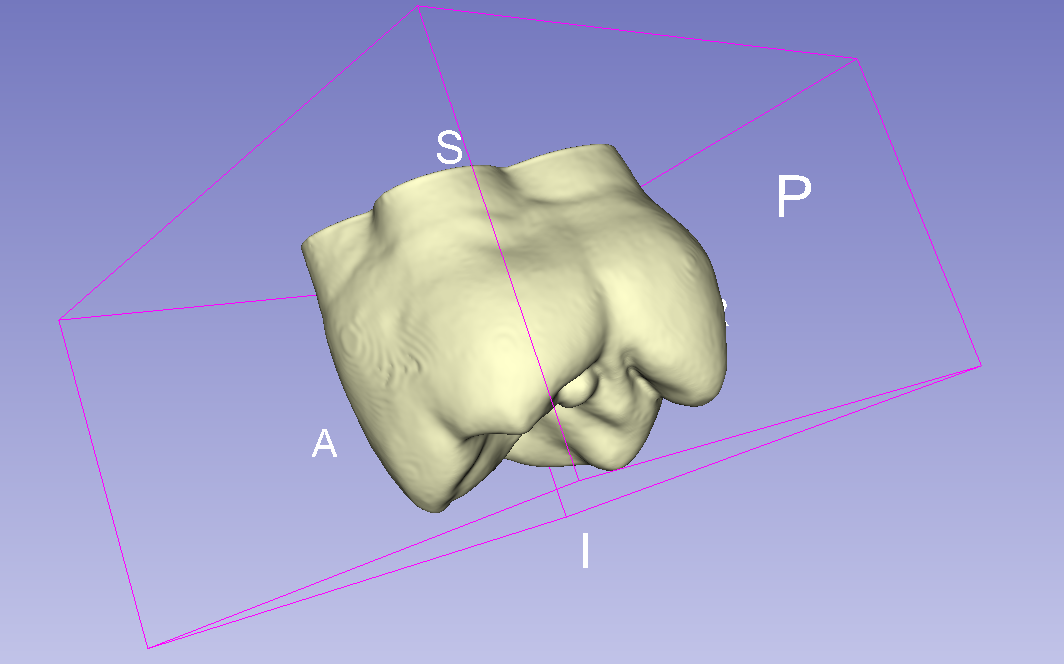
\includegraphics[width=0.5\textwidth]{img/3d_view_error.png}
	\caption{Fehlerhafte Segmentierung einer CT-Aufnahme im Format \ac{8UInt}}
	\label{fig:3d_error}
\end{figure}

Zu sehen ist ein 3D Modell, das nur aus einem Segment besteht. In diesem Fall
wurde der gesamte Zahn mit Pulpa als Dentin markiert. Nach einer etwas detaillierteren
Analyse konnte festgestellt werden, dass das Problem wohl im Bereich der
Auffüllung liegt. Den Grund dafür liefern die einzelnen Datensätze während der Segmentierung.
Betrachtet man diese genauer so fällt auf, das der Zahn zu Beginn richtig segmentiert
wird, auch ohne die Pulpa. Nachdem dann die Auffüllung über das Bild läuft, wird
diese zuerst richtige Segmentierung wieder verworfen.

Durch diese Limitierung ergibt sich eine weitere. Zu Beginn in der Analysephase des
Projektes, war eine Vorverarbeitung der Bilder vorgesehen, dass die Komprimierung
eines Bildes vornimmt und so die Bilder deutlich handlicher macht. Das Verfahren
hierzu wurde in Kapitel \ref{subsec:datensätze} erläutert. Da dieses Verfahren allerdings
einen Formatwechsel von \ac{16Int} nach \ac{8UInt} bewirkt und diese Bilder nicht
richtig segmentiert werden können, scheidet die Vorverarbeitung von Bildern aus.

Eine weitere Limitierung der Software liegt im Batch Modus. Wird ein Batch Modus
ausgeführt, so werden im Anschluss die Bilder nicht in die Szene geladen. Dies muss
manuell erfolgen über den Import des Kernsystems. Soll für die unterschiedlichen
Bilder ein \ac{3D} Modell erzeugt werden müssen diese ebenfalls manuell als Segmentierung
geladen werden. Diesem Verhalten könnte man mit einer einfache Checkbox
entgegenwirken, indem man die Checkbox setzt, wenn man nach dem Batch alle
Bilder laden möchte.

Zuletzt sei noch auf eine Limitierung hingewiesen, die der Erweiterbarkeit des Moduls
dient. Soll die Erweiterung um zusätzliche Funktionen erweiter werden, dann sind
kleine Änderungen in einer bestehenden Klasse notwendig. Konkret geht es hier um
die Klasse \texttt{ToothAnalyserWidget}. Hier muss je nach Ausprägung der \ac{UI}
der neuen Funktion, Methoden hinzugefügt werden. Diese Situation ist zwar entgegen
vieler Konventionen, jedoch sorgt sie auch dafür, dass die Komplexität des Quellcodes
nicht zu groß wird.

Mit der Beschreibung dieser limitierenden Faktoren wurden alle Ergebnisse, die
in dieser Arbeit erzielt wurden präsentiert. Es bleibt zum Schluss noch eine Interpretation
der Ergebnisse aus kritischer Sicht.
% ---------------------------------------------------------------------------------------